\documentclass[usegraphicx,usenatbib,referee]{mn2e}


% only needed for draft watermark
\usepackage[
    paperwidth=8.3in,
    paperheight=11.7in,
    left=0.5in,
    right=0.5in,
    top=1.5in,
    bottom=1.0in,
    hmarginratio=1:1]{geometry}

%\usepackage{draftwatermark}
%\SetWatermarkScale{5}
%\SetWatermarkLightness{0.8}


\usepackage{graphicx}
\usepackage{verbatim}
\usepackage{color}
\usepackage{xcolor}
\usepackage[normalem]{ulem} % for striking out with \sout
\usepackage{amsmath} % for boldsymbol
\usepackage{breqn}
%\usepackage{amsfonts}
\usepackage{enumitem}

%\usepackage{palatino}

% A comment block

%\newcommand{\comment}[1]{}

% For color
\newcommand{\mpname}[1]{#1_color.eps}
\newcommand{\clraitoff}{red}
\newcommand{\lumblack}{(black)}
\newcommand{\lumblue}{(blue)}
\newcommand{\lumred}{(red)}
\newcommand{\vdisred}{(red-dashed curve)}
\newcommand{\vdisblue}{(blue-solid curve)}

% For bw
%\newcommand{\mpname}[1]{#1.eps}
%\newcommand{\clraitoff}{}
%\newcommand{\lumblack}{}
%\newcommand{\lumblue}{}
%\newcommand{\lumred}{}
%\newcommand{\vdisred}{(dashed curve)}
%\newcommand{\vdisblue}{(solid curve)}

\newcommand{\umag}{$u$}
\newcommand{\gmag}{$g$}
\newcommand{\rmag}{$r$}
\newcommand{\imag}{$i$}
\newcommand{\zmag}{$z$}
\newcommand{\gmr}{$g-r$}



\newcommand{\gammat}{$\gamma_T$}
\newcommand{\gammacross}{$\gamma_\times$}
\newcommand{\deltasig}{$\Delta \Sigma$}
\newcommand{\deltaplus}{$\Delta \Sigma_+$}
\newcommand{\deltacross}{$\Delta \Sigma_\times$}
\newcommand{\deltarho}{$\Delta \rho$}
\newcommand{\movr}{$M(<r)$}
\newcommand{\sigmacrit}{$\Sigma_{crit}$}

\newcommand{\photoz}{photo-z}
\newcommand{\photozs}{photo-zs}

\newcommand{\tlum}{$L^{tot}$}
\newcommand{\tngal}{$N_{gal}^{tot}$}

\newcommand{\lstarlim}{$0.4 L_*$}
\newcommand{\lvir}{$L_{200}$}
\newcommand{\nvir}{$N_{200}$}
\newcommand{\rvir}{$r_{200}^{gals}$}

\newcommand{\ngal}{$N_{gal}$}
\newcommand{\maxbcg}{maxBCG}
\newcommand{\numNgalBins}{12}
\newcommand{\numLumBins}{16}

\newcommand{\tngalAperture}{2$h^{-1}$ Mpc}

\newcommand{\photo}{\texttt{PHOTO}}
\newcommand{\astrop}{\texttt{ASTRO}}
\newcommand{\mt}{\texttt{MT}}
\newcommand{\spectro}{\texttt{SPECTRO}}
\newcommand{\spectroone}{\texttt{SPECTRO1d}}
\newcommand{\spectrotwo}{\texttt{SPECTRO2d}}
\newcommand{\target}{\texttt{TARGET}}

\newcommand{\lenszmax}{0.3}
\newcommand{\lenszmin}{0.05}

\newcommand{\photoversion}{\texttt{v5\_4}}

%\def\eone{e$_1$}
%\def\etwo{e$_2$}
\newcommand{\etan}{e$_+$}
\newcommand{\erad}{e$_\times$}
\newcommand{\eclass}{\texttt{ECLASS}}
\newcommand{\eclasscut}{-0.06}
\newcommand{\gmrcut}{0.7}

\newcommand{\hrs}{$^{\mathrm h}$}
\newcommand{\minutes}{$^{\mathrm m}$}

\newcommand{\ugriz}{$u, g, r, i, z$}
\newcommand{\polarization}{polarization}

\newcommand{\wgm}{$w_{gm}$}
\newcommand{\wgg}{$w_{gg}^p$}
\newcommand{\wmm}{$w_{mm}$}
\newcommand{\xigg}{$\xi_{gg}$}
\newcommand{\ximm}{$\xi_{mm}$}
\newcommand{\xigm}{$\xi_{gm}$}

\newcommand{\numspec}{127,001}
\newcommand{\numspecvlim}{10,277}
\newcommand{\numrand}{1,270,010}
\newcommand{\numspectot}{278,192}
\newcommand{\numvdis}{49,024}
%\newcommand{\numsource}{10,259,949}
% hirata: 
\newcommand{\nummask}{1,815,043}
\newcommand{\numTenMpc}{132,473}
\newcommand{\numThirtyMpc}{101,221}
\newcommand{\numsource}{27,912,891}

\newcommand{\numpairsTenMpc}{2,670,898,177}
\newcommand{\altnumpairsTenMpc}{2.7 billion}
\newcommand{\numpairsThirtyMpc}{14,818,082,122}
\newcommand{\altnumpairsThirtyMpc}{14.8 billion}



\newcommand{\xirmax}{$\xi_{gm}(R_{max})$}


\def\eps@scaling{1.0}% 

\newcommand{\snr}{$S/N$}
\newcommand{\hlr}{$r_{50}$}
\newcommand{\hlrmean}{1.54}
\newcommand{\hlrwidth}{1.00}

\newcommand{\psffwhmmean}{3.660}
\newcommand{\psffwhmwidth}{0.377}

\newcommand{\nmasks}{1400}
\newcommand{\uberseg}{{\"u}berseg}

% stolen from the BA14 source
\newcommand{\vecg}{\mbox{\boldmath $g$}}
\newcommand{\vecD}{\mbox{\boldmath $D$}}
\newcommand{\vecQ}{\mbox{\boldmath $Q$}}
\newcommand{\matR}{\mbox{$\bf R$}}
\newcommand{\matC}{\mbox{$\bf C$}}
\newcommand{\bnabg}{ \boldsymbol{\nabla_g}}

\newcommand{\desreq}{$4\times 10^{-3}$}
\newcommand{\lsstreq}{$2\times 10^{-3}$}


\newcommand{\mnras}{MNRAS}%
\newcommand{\apj}{ApJ}%
\newcommand{\apjs}{ApJS}%
\newcommand{\aj}{AJ}%
\newcommand{\pasp}{PASP}%
\newcommand{\jcp}{J.~Chem.~Phys.}
\newcommand{\aaps}{AASP}
\newcommand{\aap}{AAP}

\newcommand{\est}{$e$}
\newcommand{\mest}{e}

\newcommand{\mcal}{metacalibration}
\newcommand{\Mcal}{Metacalibration}
\newcommand{\mcalR}{$R$}
\newcommand{\mcalRmean}{$\langle R \rangle$}
\newcommand{\mcalRpsf}{$R^{p}$}
\newcommand{\mcalRpsfnoise}{$R^{p}_\eta$}
\newcommand{\mcalRo}{$R_o$}
\newcommand{\mcalRnoise}{$R_\eta$}

\newcommand{\mcalRg}{$R_{\gamma}$}
\newcommand{\mcalRS}{$R_{S}$}
\newcommand{\mcalRgmean}{$\langle R_{\gamma} \rangle$}
\newcommand{\mcalRSmean}{$\langle R_{S} \rangle$}

\newcommand{\mcalRtwopt}{$R^{2pt}$}
\newcommand{\mcalRtwoptmean}{$\langle R^{2pt} \rangle$}


\newcommand{\mcalRmodel}{$R^{model}$}
\newcommand{\mcalRnoisemodel}{$R^{model}_\eta$}

\newcommand{\probe}{$P(e_\alpha e_\beta)$}


\newcommand{\nsimShear}{0.02,0.00}
\newcommand{\nsimNgal}{$10^8$}
\newcommand{\nsimNgalTwo}{$2 \times 10^8$}
\newcommand{\nsimNgalFour}{$4 \times 10^8$}
\newcommand{\nsimNgalBD}{$5.6 \times 10^9$}
\newcommand{\nsimNStar}{$5.6 \times 10^8$}
\newcommand{\nsimNstarperc}{10\%}
\newcommand{\starnoiseincrease}{$\sim 2-3$\%}

%\newcommand{\psfedist}{$(0.0,0.7) \pm 1.8$}
\newcommand{\nsimPSFShape}{$0.000,0.025$}

%\newcommand{\psfrdist}{log-normal $(3.66 \pm 0.38)$}
\newcommand{\psfrdist}{0.9}

\newcommand{\galrdist}{COSMOS Fits}
\newcommand{\cosmosrdist}{$1.8 \pm 0.8$}

%\newcommand{\cosmosname}{COSMOS 23.5}
\newcommand{\cosmosname}{COSMOS}

\newcommand{\detrend}{de-trending}
\newcommand{\Detrend}{De-trending}

\newcommand{\fixnoise}{\texttt{fixnoise}}

\newcommand{\ngmix}{\texttt{ngmix}}


\newcommand{\Aslope}{$-1.11$}
\newcommand{\Rcorr}{$-0.0694$}
\newcommand{\rgbias}{$(-1.6 \pm 0.5) \times 10^{-3}$}

\newcommand{\bdsim}{\texttt{BDK}}
\newcommand{\bdstar}{\texttt{BDK+Stars}}
\newcommand{\bdmask}{\texttt{Mask}}
\newcommand{\rgsim}{\texttt{RG}}
\newcommand{\pimprovement}{90}


\newcommand{\RR}{$\left<RR\right>$}
\newcommand{\RS}{$\left<RR_{S}\right>$}
\newcommand{\SSs}{$\left<R_{S}R_{S}\right>$}

%\renewcommand*\rmdefault{cmr}
%\usepackage{default}

\title{Noise Effects in \Mcal\ Weak Lensing Shear Estimation}

\author[Sheldon et al.]{Erin S. Sheldon$^1$, Eric M. Huff$^2$\\
$^1$Brookhaven National Laboratory, Bldg 510, Upton, New York 11973\\
$^2$Center for Cosmology and Astroparticle Physics, Department of Physics, The Ohio State University, OH 43210, USA }
    
%Matthew R. Becker$^2$ \\
%$^1$Brookhaven National Laboratory, Bldg 510, Upton, New York 11973\\
%$^2$Department of Physics, Stanford University, 382 Via Pueblo Mall, Stanford, CA 94305, USA}


\begin{document}

\maketitle

\begin{abstract}

We implement corrections for sheared correlated noise and selections effects in
\mcal. We explore the effects of stellar contamination and masking.   

\end{abstract}


\begin{keywords}                                                                    
    cosmology: observations,
    gravitational lensing: weak,
    dark energy
\end{keywords} 

\section{Introduction} \label{sec:intro}

\Mcal is a new technique for measuring the shear due to weak gravitational
lensing \citep{HuffMcal}.


Weak gravitational lensing has become an established technique for measuring
mass in the universe (XXX refs).  Measurement of the lensing shear effect is
core to the design of current and future imaging surveys planning to measure
cosmological parameters (XXX refs).  In order to fulfill the goals of future
surveys such as LSST, the shear effect must be measured with exquisite accuracy,
at the part in a thousand level (XXX ref).

The weak lensing shear due to a foreground lens introduces correlations in the
shapes of background galaxies at the percent level, or less (XXX cite).  There
have traditionally been two approaches to measuring this effect: measuring
moments of the light distribution and fitting models.

In the model fitting approach, a parametric model is fit to the galaxy surface
brightness profile, and the shear estimator is based on the parameters of this
model.  This method is limited for two primary reasons:  The first is that the
model must very accurately reproduce the underlying galaxy profile and shape in
order for the shear inference to be accurate (XXX ref), which requires a very
large number of parameters.  If the model cannot sufficiently reproduce the
galaxy the estimator is said to exhibit ``model bias''.  The second is that the
effect of noise on the non-linear fitting is significant for low
signal-to-noise (\snr\) images, and this effect is difficult to predict (XXX
ref).  This ``noise bias'' is exacerbated by the large number of parameters
required to represent the galaxy.

Due to these biases, model fitting methods require calibration from some
external source. Since there are no absolute calibration sources in the
universe, these methods ultimately require calibration based on simulations
(XXX ref).  These simulations must include all the relevant details of the real
universe in order to provide an accurate calibration.  As such, the science of
shear from model fitting is essentially that of accurately simulating
observations of the universe.

We not turn to moment based methods. The simplest approach to measuring shear
is to examine the unweighted second moments of the galaxy light distribution,
after correction for the effect of the point spread function (XXX ref).
However, in the presence of noise, the measurement error in these moments
diverges (XXX ref).  To address this issue a radial weight function can be
applied.

There have been a few approaches to using weighted moments.  One involves
adapting the weight function to match the object, which has the advantage of
dramatically increasing the sensitivity of the estimator to the shear compared
to a fixed weight (XXX ref). Such methods can be made quite accurate for high
\snr\ images, with little model bias (XXX ref yuki).  Another method involves
working in Fourier space, and shearing the coordinate system rather than
adapting the moment; this method does not suffer model bias because it is the
shear of the coordinate system that is iterated rather than a model for the
galaxy.  However, each of these methods suffer the ``noise bias'' found in
model fitting methods, due to the non-linear fitting involved with the
measurement. Without further development are not accurate
enough for current and future surveys (XXX ref).

Two recently introduced methods have been developed to avoid noise bias in
moment based shear inference.  The first involves measuring the moments in
Fourier space, after subtracting off the noise power spectrum.  A circular
weight is used to avoid non-linear fitting issues.  These un-normalized moments
are then summed directly to provide a shear estimator (XXX ref).  This method
has been shown to be very accurate, but because the moments are not normalized,
the weighting is essentially by flux, weighting to the brightest galaxies,
which is highly sub-optimal. Attempts to use different weighting have not
yet been demonstrated to be accurate (XXX ref).

A promising new moment based method was introduced by (XXX ref).  A rigorous
Bayesian framework was developed in which prior information on galaxy images
from a high \snr\ deep data set is combined with knowledge of how a particular
measurement (e.g. a model fit or moments) responds to the shear in the absence
of noise.  The method has been shown to be accurate enough for future surveys
in a highly controlled, but unrealistic numerical experiment using model
fitting techniques (XXX ref sheldon).  A more practical version using
un-normalized moments in Fourier spaces, similar to (XXX ref) was tested in
(XXX ref).  While the accuracy in that test fell somewhat short of the
part-in-a-thousand target, the method shows great promise, since the required
prior information from deep data should in principle be available to current
and future surveys (XXX ref).

\Mcal\ \citep{HuffMcal} is a new shear measurement technique designed to
address the shortcomings of standard shear measurement techniques.  The essence
of \mcal\ is to directly measure how a particular measurement responds to a
shear, eliminating both model bias and noise bias.

The \mcal\ technique was shown to be accurate in controlled simulations
\citep{HuffMcal}.  However, the simulations used in that study (based on those
in XXX ref) used fairly high \snr\ galaxy images, and the galaxies were
relatively large compared to the PSF size.  In a real survey, the images are
dominated by small faint galaxies.  Additionally, for low \snr\ images the
effects of correlated noise that arise in the \mcal\ procedure become
important.

In this study we introduce a simple correction for this correlated noise.
Additionally, we introduce a formalism to deal with selection effects, for
example cuts on \snr\ and galaxy size, that are required for any practical
analysis.  We additionally examine the effects of stellar contamination and
missing data.  We show that, in all scenarios we tested, \mcal\ is sufficiently
accurate for current and future studies.

Say where things are.


\section{Metacalibration} \label{sec:mcal}

In this section we introduce the basic concepts of \mcal. We will derive the
full formalism for shear measurements in \S \ref{sec:selection}.

Suppose we have a biased shear observable \est, which may be some estimate of
an objects ellipticity. We can expand this observable in a Taylor
series about zero shear
\begin{align} \label{eq:Eexpand}
    \mest(\gamma) &= \mest|_{\gamma=0} + \gamma ~ \frac{ \partial \mest }{ \partial \gamma }\bigg|_{\gamma=0}  + ... \nonumber \\
                  &= \mest|_{\gamma=0} + \gamma \mbox{\mcalR} + ...
\end{align}
where we have defined the shear response:
\begin{align}
    \mbox{\mcalR} &\equiv \frac{\partial \mest}{\partial \gamma} \bigg|_{\gamma=0}.
\end{align}
We can use the ensemble mean of such measurements as a shear estimator:
\begin{align}
    \langle \mest \rangle &= \langle \mest \rangle |_{\gamma=0} + \langle \gamma \mbox{\mcalR} \rangle + ... \nonumber \\
                          &\approx \langle \gamma \mbox{\mcalR} \rangle
\end{align}
where we have assumed the intrinsic ellipticities of galaxies are
randomly oriented such that $\langle \mest \rangle |_{\gamma=0} = 0$.
If we have estimates of \mcalR\ for each galaxy, we
can form a weighted average:
\begin{align}
    \langle \gamma \rangle &\approx \frac{\langle \mest \rangle}{\langle \mbox{\mcalR} \rangle} = \frac{\langle R \gamma \rangle}{\langle \mbox{\mcalR} \rangle}
\end{align}
Note the special case of constant shear, where $\gamma$ factors out
of the right hand side.

The essence of \mcal\ \citep{HuffMcal} is to estimate the shear response
\mcalR\ for a measurement \est\ directly from image data.  This is
accomplished using a numerical derivative.  The original image $I$ is
de-convolved from the point spread function (PSF), sheared, and re-convolved
by the PSF.  A slightly larger PSF is used in order to suppress modes 
exposed by the shearing that were previously hidden in the finite
resolution of the original image.  This \mcal\ process is repeated for a
positive and negative shear, which can be used to form a central derivative.
We can represent this as a series of operations on the observed image $I$:
\begin{equation}
    I(\gamma) = I \ast P^{-1} \oplus \gamma \ast P_{d}
\end{equation}
where $\ast $ represents convolution, $\oplus$ represents shearing,
and $P$ represents the point spread function.  De-convolution
is represented as ``inverse'', $P^{-1}$.  The slightly larger PSF, or
dilated PSF, is represented by $P_{d}$.

To form the central derivative we shear by a small positive and negative
amount $\gamma$
\begin{equation} \label{eq:Rnum}
    R = \frac{\mest(+\gamma) - \mest(-\gamma)}{\Delta \gamma},
\end{equation}
where $\Delta \gamma = 2\gamma$.
A re-convolved, but not sheared, image should be used
to calculate the shear estimator \mest.
%\begin{equation} \label{eq:estimator}
%    \mest = \frac{\mest(+\gamma) + \mest(-\gamma)}{2}.
%\end{equation}


%The unbiased estimator is then given by
%\begin{align}
%    \gamma = \frac{\langle \mest \rangle}{\langle \mbox{\mcalR} \rangle}.
%\end{align}

The measurement \est\ has two-components, and the response \mcalR\ is
a $2 \times 2$ matrix. Thus the mean shear is given by the matrix
equation
\begin{align}
    \gamma &= 
%    \langle \mbox{\mcalR} \rangle^{-1} \left[ \langle \mest \rangle - \langle \mbox{\mcalRpsf} \rangle \langle e^{p} \rangle \right].
    \langle \mbox{\mcalR} \rangle^{-1} \langle \mest \rangle.
\end{align}
We generally find that the off-diagonal terms of this matrix are negligible in the mean
and can be ignored.

If the PSF correction is not perfect, the leading term $\langle \mest
\rangle|_{\gamma=0}$ will not be zero.  \cite{HuffMcal} discussed another
response, the response of the measurement to the PSF ellipticity, to correct
this effect.  In this work we instead reconvolve the image by a symmetrized
version of the PSF, which removes most additive effects from the PSF  (see \S
\ref{sec:modelfit}).


\begin{comment}
This
correction involves shearing the PSF rather than the galaxy:
\begin{equation}
    \mbox{\mcalRpsf} = \frac{\mest(+\gamma^{p}) - \mest(-\gamma^{p})}{\Delta \gamma^{p}},
\end{equation}
where $\gamma^{p}$ is a shear applied to the PSF.  
This term can be subtracted to approximately correct for additive PSF errors:
\begin{equation}
    \gamma = \frac{\langle \mest \rangle - \langle \mbox{\mcalRpsf} e^{p} \rangle}{ \langle \mbox{\mcalR} \rangle}.
\end{equation}
In practice one can calculate mean responses, factoring out the response term:
\begin{equation}
    \gamma = \frac{\langle \mest \rangle - \langle \mbox{\mcalRpsf} \rangle \langle e^{p} \rangle}{ \langle \mbox{\mcalR} \rangle}.
\end{equation}
\end{comment}

In \cite{HuffMcal} a sophisticated inference was used, rather than simple
averages, in order to deal with the relatively large variance in \mcalR\
associated with the particular estimators used therein.  For the estimator
we use in this work, we find simple averages suffice.


\section{Full Formalism} \label{sec:selection}

%  ['%.1f' % (sqrt(2)*s,) for s in [7,10,13,16,19]]
%    ['9.9', '14.1', '18.4', '22.6', '26.9']

In this section we derive the full metacal formalism, including selection
effects. 

Consider a selection that modifies the distribution of the measurement \est,
which we can, without loss of generality, refer to as the ellipticity.  As
a shorthand we will write this selection function as $S(\mest)$, the probability of
selecting an object with ellipticity \est, although the selection may be
indirect, for example a cut on \snr.  This selection function could also
represent some kind of weighting scheme.

We introduce the following notation regarding the shear estimator and the
selection function:  We write the sheared version of the ellipticity as
$\mest^+$ and $\mest^-$, for measurements on positive and negatively sheared
images respectively.  Similarly, we can select objects based on sheared
parameters, which we denote $S^+$ and $S^-$, the probability of
selection after a positive or negative shear is applied, respectively.

\subsection{Response for the Mean Shear} \label{sec:Rmean}

The mean ellipticity over an ensemble can be written as 
\begin{align}
    \langle \mest \rangle = \int P(\mest)~\mest~d\mest,
\end{align}
where $P(\mest)$ is the probability distribution.  If we introduce
a selection, the mean becomes
\begin{align}
    \langle \mest S \rangle = \int S(\mest)~P(\mest)~\mest~d\mest.
\end{align}
We will assume the $\int de P(\mest) S(\mest) = 1$.

Assuming galaxy orientations are random in the absence of shear, 
the mean ellipticity can be rewritten, to leading order, as
\begin{align}
    \langle eS \rangle \approx \int de \gamma \frac{\partial S(\mest) P(\mest) \mest  }{\partial \gamma}\bigg|_{\gamma=0} d\mest = \langle \gamma R \rangle,
\end{align}
where we have ignored the perturbation of the normalization $\int de P(e)S(e)$,
because it leads to terms that are second order in the shear.
The mean shear is thus weighted by a response term \mcalR.  If
the \mcalR\ are known, we can form a weighted average estimator
for the shear:
\begin{align}
    \gamma \approx \frac{\left< e \right>}{\mbox{\mcalRmean}}
\end{align}

We can calculate this response using quantities measured on artifically
sheared images, as presented in \S \ref{sec:mcal}
\begin{align}
    \mbox{\mcalRmean}  &= \int \frac{\partial S(\mest) P(\mest) \mest  }{\partial \gamma}\bigg|_{\gamma=0} d\mest \nonumber \\
    &= \int \left[ S(\mest) P(\mest) \frac{\partial \mest}{\partial \gamma}\bigg|_{\gamma=0} + \mest \frac{\partial P(\mest) S(\mest)}{\partial \gamma}\bigg|_{\gamma=0} \right] d\mest
\end{align}
We will approximate the derivatives using finite differences in the shear.
Using the notation for measurements on sheared images, introduced
in \S \ref{sec:selection}, we can rewrite the response as
\begin{align} \label{eq:Rmean}
    \mbox{\mcalRmean} &\approx
    \int d\mest \left [ S P \left( \frac{ \mest^+ - \mest^- }{\Delta \gamma}\right) + \mest \left( \frac{ P^+ S^+ - P^- S^- }{\Delta \gamma}\right) \right] d\mest \nonumber \\
    &=\frac{\langle \mest^+ S \rangle - \langle \mest^- S \rangle}{\Delta \gamma} + 
\frac{\langle \mest S^+ \rangle - \langle \mest S^- \rangle}{\Delta \gamma} \nonumber \\
       &\equiv \langle \mbox{\mcalRg} \rangle + \langle \mbox{\mcalRS} \rangle
\end{align}
The first term \mcalRgmean\ is average of the shear responses measured for
individual galaxies, as discussed in  \S \ref{sec:mcal}.
Selections are based on the unsheared object parameters.

The second term \mcalRSmean\ represents the response of the mean ellipticity to
selections.  The $\langle \mest S^+ \rangle$ represents the mean of the
unsheared ellipticities, with selection based on the sheared parameters, and
$\langle \mest S^- \rangle$ represents the mean of the unsheared ellipticities,
with selection based on the negatively sheared parameters.


%The $\langle \mest^+ S \rangle$ represents the mean of the positively sheared
%ellipticities, with selection based on the unsheared parameters. The $\langle
%\mest^- S \rangle$ represents the mean of the negatively sheared ellipticities,
%with selection based on the unsheared parameters.


Thus in order to produce a mean shear measurement, one measures the
average ellipticity $\langle e S \rangle$, the mean of the individual galaxy
shear responses \mcalRgmean, the mean ellipticity after selections based on
positively sheared images $\langle e S^+ \rangle$,and the mean ellipticity
after selections based on negatively sheared images $\langle e S^- \rangle$.


Note, in the above selections that produce additive effects are not addressed.
If the PSF is symmetrized, as we will do (see \S \ref{sec:modelfit}) then
selections on object properties will not correlated with the PSF shape, by
construction. Note, however, that pre-selections, for example detection
thresholds, will in general produce such biases.  We will test the importance
of this effect using image simulations.

%In practice, we recommend storing all the sheared and unsheared measurements
%and perform separate selections and statistics on those values to compute any
%ensemble averages needed for a particular inference (see e.g. \S
%\ref{sec:Rtwopt} where these quantities are used differently).

%Similar corrections can be derived for the PSF response \mcalRpsf.  For these
%terms, the psf shape in the product $\mbox{\mcalRpsf} e^p$ should be calculated
%from the unsheared data.



\subsection{Response for 2-point Functions} \label{sec:Rtwopt}

We can extend this formalism to 2-point functions, which we will write
as
\begin{align}
    \xi &= \langle e_\alpha e_\beta \rangle \nonumber \\
        &= \int \mbox{\probe} e_\alpha e_\beta d e_\alpha d e_\beta
\end{align}
where the indices $\alpha, \beta$ indicate the ellipticity for two different
objects or regions of sky.  Including selection effects, this becomes
\begin{align}
    \xi &= \int \mbox{\probe} S_\alpha S_\beta e_\alpha e_\beta d e_\alpha d e_\beta
\end{align}
where the selections are independent on each object.

Adopting the symmetry assumptions used in \S \ref{sec:Rmean}, and additionally that
the mean shear is zero over a large area of sky used to measure
the 2-point function, the leading
term in the Taylor expansion is a second derivative
\begin{align} \label{eq:basictwopt}
%    \xi \approx \left< \gamma_\alpha \gamma_\beta   \frac{\partial^2 \xi}{\partial \gamma_\alpha \partial \gamma_\beta}\bigg|_{\gamma=0} \right> \equiv \left< \gamma_\alpha \gamma_\beta \mbox{\mcalRtwopt} \right>.
\xi \approx \int d e_\alpha  de_\beta  \gamma_\alpha \gamma_\beta \frac{\partial^2 S_\alpha S_\beta \mbox{\probe} e_\alpha e_\beta}{\partial \gamma_\alpha \partial \gamma_\beta}\bigg|_{\gamma=0}  \equiv \left< \gamma_\alpha \gamma_\beta \mbox{\mcalRtwopt} \right>.
\end{align}
The next largest terms are of order $ \langle e_\alpha \rangle|_{\gamma=0} \gamma_\alpha^2$.
In equation \ref{eq:basictwopt} the
true correlation function has been weighted by a response, where the response
is given by
\begin{align}
%    \mbox{\mcalRtwoptmean} = \left< \frac{\partial^2 \xi}{\partial \gamma_\alpha \partial \gamma_\beta}\bigg|_{\gamma=0} \right> = 
    \mbox{\mcalRtwoptmean}  = 
    \int d e_\alpha  de_\beta  \frac{\partial^2 S_\alpha S_\beta \mbox{\probe} e_\alpha e_\beta}{\partial \gamma_\alpha \partial \gamma_\beta}\bigg|_{\gamma=0}.
\end{align}
If we know the responses, we can form an estimator for the correlation function
that takes the form of a weighted average:
\begin{align}
    \xi \approx \frac{\langle \gamma_\alpha \gamma_\beta R^{2pt} \rangle}{\langle R^{2pt}\rangle}.
\end{align}

Note the probability distribution \probe\ is joint in the two ellipticities
because the shear at each galaxy $\alpha$ is correlated with that at galaxy
$\beta$. Assuming the shapes of galaxies are not correlated in the absence of
shear, \probe\ is separable at zero shear such that $\mbox{\probe}|_{\gamma=0}
= P(e_\alpha)|_{\gamma=0} P(e_\beta)|_{\gamma=0}$.  The following identities
also hold:
\begin{align}
    \frac{\partial \mbox{\probe}}{\partial \gamma_\alpha}\bigg|_{\gamma=0} &= P(e_\beta) \frac{\partial P(e_\alpha) }{\partial e_\alpha} \frac{\partial e_\alpha}{\partial \gamma_\alpha}\bigg|_{\gamma=0} \nonumber \\
    \frac{\partial^2 \mbox{\probe}}{\partial \gamma_\alpha \partial \gamma_\beta}\bigg|_{\gamma=0} &= \frac{\partial P(e_\alpha) }{\partial e_\alpha} \frac{\partial P(e_\beta) }{\partial e_\beta}  \frac{\partial e_\alpha}{\partial \gamma_\alpha} \frac{\partial e_\beta}{\partial \gamma_\beta}\bigg|_{\gamma=0}.
\end{align}
It then follows that the response can be completely factored such that
\begin{align}
    \int d e_\alpha  de_\beta  \frac{\partial^2 S_\alpha S_\beta \mbox{\probe} e_\alpha e_\beta}{\partial \gamma_\alpha \partial \gamma_\beta}\bigg|_{\gamma=0} 
      &\approx \int d e_\alpha  \frac{\partial S_\alpha P(e_\alpha) e_\alpha}{\partial \gamma_\alpha}\bigg|_{\gamma=0} de_\beta   \frac{\partial S_\beta P(e_\beta) e_\beta}{\partial \gamma_\beta}\bigg|_{\gamma=0} \nonumber \\
      &=  \left< R_\alpha \right> \left< R_\beta \right>.
\end{align}
These two responses $\left< R_\alpha \right>$ and $\left< R_\beta \right>$ are statistically identical, and are each equal to the
response of the mean shear given in equation \ref{eq:Rmean}.  Thus the
response of the two-point function is approximately given by
\begin{align}
    %\left< R^{2pt} \right> = \left< \frac{\partial^2 \xi}{\partial \gamma_\alpha \partial \gamma_\beta}\bigg|_{\gamma=0} \right> \approx \mbox{\mcalRmean}^2.
    %\left< \frac{\partial^2 \xi}{\partial \gamma_\alpha \partial \gamma_\beta}\bigg|_{\gamma=0} \right> \approx \mbox{\mcalRmean}^2.
    \left< R^{2pt} \right> \approx \mbox{\mcalRmean}^2.
\end{align}
We can form a simple estimator for the 2-point function as:
\begin{align}
    \xi \approx \frac{ \langle e_\alpha e_\beta \rangle }{\mbox{\mcalRmean}^2}.
\end{align}

In what follows we test the formulas for mean shear.  We will test the
response for 2-point functions in a future work.


\subsection{Remarks on Selections}

It is important that the selections be placed well above any detection
thresholds, such that, after shearing, detected objects can move into and out
of the selected sample.  If the selection were too close to a detection
threshold, some objects that should become detectable after
a shear would not be included.

In real data, a selection may directly or indirectly select the redshift of the
sources, which means the true shear will be different after selection, even in
the absence of selection biases.  This must be taken into account separately.
We will not treat this effect in what follows.  TODO estimate size of this
effect



\begin{comment}
\subsubsection{Without the factorization}

We can expand this response as
\begin{align} \label{eq:twoptres1}
    \bigg< \frac{\partial^2 \xi}{\partial \gamma_\alpha \partial \gamma_\beta}&\bigg|_{\gamma=0} \bigg> =
          \int d e_\alpha  de_\beta  \biggl[S_\alpha S_\beta \frac{\partial^2 P_{\alpha\beta} e_\alpha e_\beta}{\partial \gamma_\alpha \partial \gamma_\beta}   \nonumber \\
         & + S_\alpha \frac{\partial S_\beta}{\partial \gamma_\beta} \frac{\partial P_{\alpha\beta} e_\alpha e_\beta}{\partial \gamma_\alpha}
         + S_\beta \frac{\partial S_\alpha}{\partial \gamma_\alpha} \frac{\partial P_{\alpha\beta} e_\alpha e_\beta}{\partial \gamma_\beta} \nonumber  \\
         & + \frac{\partial S_\alpha}{\partial \gamma_\alpha} \frac{\partial S_\beta}{\partial \gamma_\beta} P_{\alpha \beta} e_\alpha e_\beta \biggr]\bigg|_{\gamma=0}  \nonumber \\
     & \equiv  \mbox{\RR} + 2 \mbox{\RS} +  \mbox{\SSs}
\end{align}
where the trailing evaluation at $\gamma=0$ is meant to apply to all the
derivatives within the brackets. Note the second and third terms are equal
under swapping of the indices and thus can be combined.


%\begin{align} \label{eq:twoptres1}
%     \left < \frac{\partial^2 \xi}{\partial \gamma_\alpha \partial \gamma_\beta}\bigg|_{\gamma=0} \right> =
%         & \int d e_\alpha  de_\beta  \biggl[ \nonumber \\
%         & \frac{\partial S_\alpha}{\partial \gamma_\alpha} \frac{\partial S_\beta}{\partial \gamma_\beta} P_{\alpha \beta} e_\alpha e_\beta  \nonumber \\
%        & + S_\alpha \frac{\partial S_\beta}{\partial \gamma_\beta} \frac{\partial P_{\alpha\beta} e_\alpha e_\beta}{\partial \gamma_\alpha} \nonumber  \\
%        & + S_\beta \frac{\partial S_\alpha}{\partial \gamma_\alpha} \frac{\partial P_{\alpha\beta} e_\alpha e_\beta}{\partial \gamma_\beta} \nonumber  \\
%        & + S_\alpha S_\beta \frac{\partial^2 P_{\alpha\beta} e_\alpha e_\beta}{\partial \gamma_\alpha \partial \gamma_\beta}  \biggr]\bigg|_{\gamma=0} \nonumber \\
%        \equiv \left<SS\right> + 2 \left<SR\right> + \left<RR\right>
%\end{align}


The first term \RR\ in equation \ref{eq:twoptres1} represents the response of
the estimator to shearing of either object in the product.  The last term \SSs\
represents the effects of independent selections in each object.  The cross
term \RS\ represent the response to shearing in one object and selection in another.

We can compute these terms using the sheared measurements, and using selections
on sheared measurements. We can approximate the derivatives with
finite differences.  The first term can be written as
\begin{align}
    \mbox{\RR} = \int d e_\alpha  d e_\beta S_\alpha S_\beta & \frac{\partial^2 P_{\alpha\beta} e_\alpha e_\beta}{\partial \gamma_\alpha \gamma_\beta} \bigg|_{\gamma=0} \approx \nonumber \\
    \frac{1}{\Delta \gamma^2} \Bigl(  & \left< S_\alpha S_\beta e_\alpha^+ e_\beta^+ \right> - \left< S_\alpha S_\beta e_\alpha^+ e_\beta^- \right> \nonumber \\
                                    - & \left< S_\alpha S_\beta e_\alpha^- e_\beta^+ \right> + \left< S_\alpha S_\beta e_\alpha^- e_\beta^- \right> \Bigr)
\end{align}
Note the cross terms are equal.  Also note we can write the 
the finite difference derivative response term
for an individual object as
$R_\alpha = (e_\alpha^+ - e_\alpha^-)/\Delta \gamma$.
Because all terms are selected based on the unsheared
parameters, we can refactor this entire term as a cross-correlation
of the individual response terms
\begin{align}
    \mbox{\RR} \approx \langle S_\alpha S_\beta R_\alpha R_\beta \rangle.
\end{align}

We can follow the same procedure for the cross term \RS, expanding the
deriviatives as finite differences:
\begin{align}
    \mbox{\RS} = \int d e_\alpha  d e_\beta  2 S_\alpha \frac{\partial S_\beta}{\partial \gamma_\beta} & \frac{\partial P_{\alpha\beta} e_\alpha e_\beta}{\partial \gamma_\alpha} \bigg|_{\gamma=0} \approx \nonumber  \\
    \frac{2}{\Delta \gamma^2} \Bigl( & \left< S_\alpha S_\beta^+ e_\alpha^+ e_\beta \right> - \left< S_\alpha S_\beta^+ e_\alpha^- e_\beta \right> \nonumber \\
    & - \left< S_\alpha S_\beta^- e_\alpha^+ e_\beta \right> + \left< S_\alpha S_\beta^- e_\alpha^- e_\beta \right> \Bigr).
\end{align}
As discussed in \S \ref{sec:Rmean}, $S^+$ and $S^-$ mean selection on
quantities measured from positively sheared and negatively sheared images,
respectively.  This term can also be further simplified in terms of the
individual shear responses $R_\alpha$.
\begin{align}
    \mbox{\RS}  \approx 
    \frac{2}{\Delta \gamma} \Bigl( & \left< S_\alpha S_\beta^+ e_\beta R_\alpha \right> - \left< S_\alpha S_\beta^- e_\beta R_\alpha \right> \Bigr).
\end{align}
Calculation of \RS\ involves two cross-correlations, with one of
the catalogs selected on sheared or unsheared parameters.

The last term \SSs\ can be written as
\begin{align}
    \mbox{\SSs} = & \int d  e_\alpha  d e_\beta  \frac{\partial S_\alpha}{\partial \gamma_\alpha} \frac{\partial S_\beta}{\partial \gamma_\beta}  P_{\alpha \beta} e_\alpha e_\beta \bigg|_{\gamma=0} \approx \nonumber \\
    & \frac{1}{\Delta \gamma^2} \Big< \left(S_\alpha^+ - S_\alpha^- \right) \left(S_\beta^+ - S_\beta^- \right) e_\alpha e_\beta  \Big> = \nonumber \\
    & \frac{1}{\Delta \gamma^2} \Big( \left< S_\alpha^+ S_\beta^+ e_\alpha e_\beta \right> - 2 \left< S_\alpha^- S_\beta^+ e_\alpha e_\beta \right> + \left< S_\alpha^- S_\beta^- e_\alpha e_\beta \right>     \Big)
\end{align}
There are three separate measurements to be made for \SSs:  the first and
last are auto-correlations where selections are placed on the positively and
negatively sheared parameters, respectively.  The second is a cross correlation
between one catalog selected using positively sheared quantities, the other
using negatively sheared quantities.
\end{comment}


\section{Contamination of the Response by Correlated Noise} \label{sec:contam}

In the presence of noise, the observed image can be written $I_o=I+\eta$, where $\eta$
is the ``noise image''.  The \mcal\ sheared images $I_o(\gamma)$ will contain
contributions from de-convolved, sheared and re-convolved noise:
\begin{align}
    I_{o}(\gamma) &= (I + \eta) \ast P^{-1} \oplus \gamma \ast P_{d} \nonumber \\
    &= I(\gamma) + \eta(\gamma).
\end{align}
The de-convolution correlates the noise across the image.  This correlated
noise is sheared, and then re-convolved by the dilated PSF, producing the
sheared correlated noise image $\eta(\gamma)$.  The pattern of this sheared
noise is coherent between the positively sheared and negatively sheared images.
The effect is small, but is amplified due to division by $\Delta \gamma$ to
form the central derivative.  We thus expect the observed response \mcalRo\ to
be contaminated by the response of the correlated, sheared noise which
we will denote \mcalRnoise:
\begin{equation}
    \mbox{\mcalRo}  =  R + \mbox{\mcalRnoise}.
\end{equation}

%A correction is also required for the PSF response term \mcalRpsf.  We find
%this correction is similar in magnitude to the correction for \mcalR, although
%it is somewhat suppressed in the final estimator due to multiplication by $e^p$.

\subsection{Expected Scaling of the Bias with Noise Level} \label{sec:scaling}

The bias in the ellipticity due to correlated noise should scale
with the noise correlation function, and thus the square of the noise level in
the image $n^2$ \citep{HirataCorrNoise}.  As stated above, this same bias will
propagate into the response.  We can write the observed \mcalRo\ as a contribution
from both the actual response \mcalR\ and a noise term \mcalRnoise\
\begin{align} \label{eq:scaling}
    \mbox{\mcalRo} &= R + \mbox{\mcalRnoise}  \nonumber \\
                   &= R + A n^2.
\end{align}


\section{Correction for Sheared, Correlated Noise} \label{sec:corr}

\begin{comment}
For shear estimators based on raw moments, without any form of iteration
or fitting, it would be sufficient to simply measure the moments of example
sheared correlated noise fields and subtract the mean response from the
responses measured on the real images.  Multiple realizations can be generated
for each galaxy to increase precision.
\end{comment}

The coefficient $A$ in Equation \ref{eq:scaling} can be calculated in simple
scenarios, as shown in \cite{HirataCorrNoise}.  However, the calculation is
more complex when modeling the effect of the PSF.  We instead explored four
different empirical corrections.  We describe our favored method
below; the others are described in appendix \ref{sec:altcorr}.

\begin{comment}
There are advantages to forward modeling which we would like to retain: the
noise in \mcalR\ using our forward-modeling approach is an order of magnitude
smaller than that seen for the re-Gaussianization approach in \cite{HuffMcal}.
In particular we find that applying smooth priors on the model parameters,
which is natural in a forward-modeling approach, stabilizes the fit and results in
a large reduction in variance.  This reduction in noise facilitates the simple
inference method outlined in \S \ref{sec:mcal}.  The failure rate is also
dramatically decreased when applying smooth priors:  we find a failure rate of
$\sim$0.003\%, as opposed to $\sim$6\% for the re-Gaussianization code
implemented in the GALSIM package \citep{GALSIM2015}.  For these reasons we
explore a simple empirical correction in the following section.
\end{comment}

\subsection{Adding a Canceling Correlated Random Noise Field} \label{sec:fixnoise}

This method, which we refer to as ``\fixnoise'', is designed to statistically
cancel the effects of correlated noise caused by the \mcal\ procedure.  For each
image that was passed through the convolution and shearing steps, producing
an image $I(\gamma)_o$, we generated a random noise field
$\tilde{\eta}$, and applied the same operations but using a shear with
the opposite sign:
\begin{equation}
    \tilde{\eta}(-\gamma) = \tilde{\eta} \ast P^{-1} \oplus (-\gamma) \ast P_{d}.
\end{equation}
We then added this image to the $I(\gamma)_o$ image.
The result, $\tilde{I}(\gamma)$, is an approximation for the image
without correlated noise:
\begin{equation}
    \tilde{I}(\gamma) = I_o(\gamma) + \tilde{\eta}(-\gamma).
\end{equation}
We used these $\tilde{I}(\gamma)$ to measure the shapes and responses used in
shear recovery.  For a single image, this procedure will not exactly cancel the
correlated noise, because the original and added noise fields are not
identical; rather the effect should cancel when averaged over a large ensemble
of galaxies.

This procedure necessarily increases the noise in the shear recovery.  Thus,
both the response and estimator should be measured on the $\tilde{I}(\gamma)$
images, so that the response is representative of the correct noise level.  To
reduce the noise in the fits, multiple randomized noise fields could be
generated and fit, and the results averaged.  This would improve the precision,
at the cost of increased computation time.

An alternative version of this method is to shear the noise exactly as the
original image is sheared, but then rotate by 90 degrees before adding.  This
version has the advantage of working even when the transformation between sky
and image involves a shear of the coordinate system\footnote{M. Jarvis, private
communication}. We will explore this method in a future work.

\section{Weighted Averages for Associated Parameters} \label{sec:weighting}

As discussed in \S \ref{sec:selection}, if a shear estimator has
non-unity response, the mean shear (or 2-point function) is effectively
weighted.  If we know the responses we can form a weighted average.

This means that associated quantities, such as average redshift, should also be
weighted by these responses.  For example, a quantity $x$ would be averaged
as
\begin{align}
    \left< x \right> = \frac{\sum_i R_i x_i}{\sum R_i}.
\end{align}
The responses are not scalar, but it is probably sufficient
to use the average of the two diagonal components of the $R$ matrix
for this purpose. One concern is that the measured $R$ values are not
strictly positive.  It is worth exploring whether this causes
any bias in real scenarios.

\section{Image Simulations} \label{sec:sims}

\subsection{Simulations with Parametric Models} \label{sec:bdsim}

We applied \mcal\ to a set of image simulations.  For the first set of
simulations we used complex parametric models.  We modeled galaxies as a bulge
and disk, with additional knots of star formation; we label this simulation
\bdsim.  We used different ellipticities for the bulge and disk components, but
gave both bulge and disk the same half light radius \hlr.

We drew the \hlr\ and flux from fits to the 25.2 magnitude limited
sample from the COSMOS data, as distributed with the GALSIM simulation package
\citep{GALSIM2015}.  In order to avoid repeating the exact parameters, we
interpolated the joint \hlr-flux distribution using a kernel density 
estimate.

The ellipticities were drawn from the simple model used in \cite{ba14}
\begin{align}
    P(e) &\propto \left[1-(e)^2\right]^2 \exp\left[-e^2/2\sigma^2\right],
\end{align}
with $\sigma=0.2$ for the disk and $\sigma=0.1$ for the bulge.  Note, we use
the ``reduced-shear'' style ellipticity, which differs by roughly a factor of
two compared to the ellipticity used in \citet{bfd2015}.

For the simulated knots of star formation, we distributed 100 point sources
according to a random walk starting at the disk centroid, with each point
taking 40 steps.  We then sheared this distribution using the same ellipticity
assigned to the disk; but note this does not result in a purely elliptical
distribution of point sources\footnote{This random walk method was inspired by
\cite{Zhang2008FourierQuadI}, but was implemented from scratch by the authors
as a GALSIM object class \texttt{galsim.RandomWalk}}.

The fraction of the flux in the bulge was drawn uniformly between zero and
unity.  The fraction of the disk flux assigned to knots of star formation
was then also chosen uniformly between zero and unity.  The resulting 
objects range from pure bulge, bulge+disk, pure disks, bulges+disk+knots, 
to pure knots, which resemble irregular galaxies.

Finally, the entire composite bulge+disk+knots object was sheared with
$g1=0.02$ in reduced shear units.

We convolved the galaxy images with a PSF modeled as a Moffat profile
\citep{Moffat1969}, with $\beta=3.5$ and FWHM=0.9 arcsec. The PSF ellipticity was set to $g_2 = 0.025$ in reduced shear units ($e_2 =
0.05$ in units of distortion). 

These convolved objects were rendered onto 0.263 arcsec pixels and constant
Gaussian noise was added, with the same noise level used for all images.

In figure \ref{fig:parametricgals} we show some example simulated galaxies with
a range of parameters.  In order to show detailed internal structure, these
models were created to be larger than any models in the actual simulations we
ran for testing, which were mostly smaller than the PSF.


\begin{figure*}
    \centering
    \includegraphics[]{example-gals-007.eps}

    \caption{Example simulated galaxy images.  Each image is composite of a
    bulge and disk, plus knots of star formation.  The half light radius is the
    same for all components, while the fraction of light in each component
    varies.  In the upper left and upper right we show pure bulge and pure disk
    models, respectively.  In the lower left we show a disk with half the light
    in knots, and in the lower right we show a pure ``irregular'' galaxy
    composed entirely of knots.  For demonstration purposes, we here sow very
    large models to make the detailed structure visible; the galaxies used for
    our shear tests are typically much smaller than the PSF. }

	\label{fig:parametricgals}

\end{figure*}

In figure \ref{fig:psimhlrcompare} we show the distribution of \hlr\ for the
parametric galaxies, along with the \hlr\ for the PSF,
converted from FWHM.  Note most objects had \hlr\ significantly smaller than
the PSF.

\begin{figure}
    \centering
    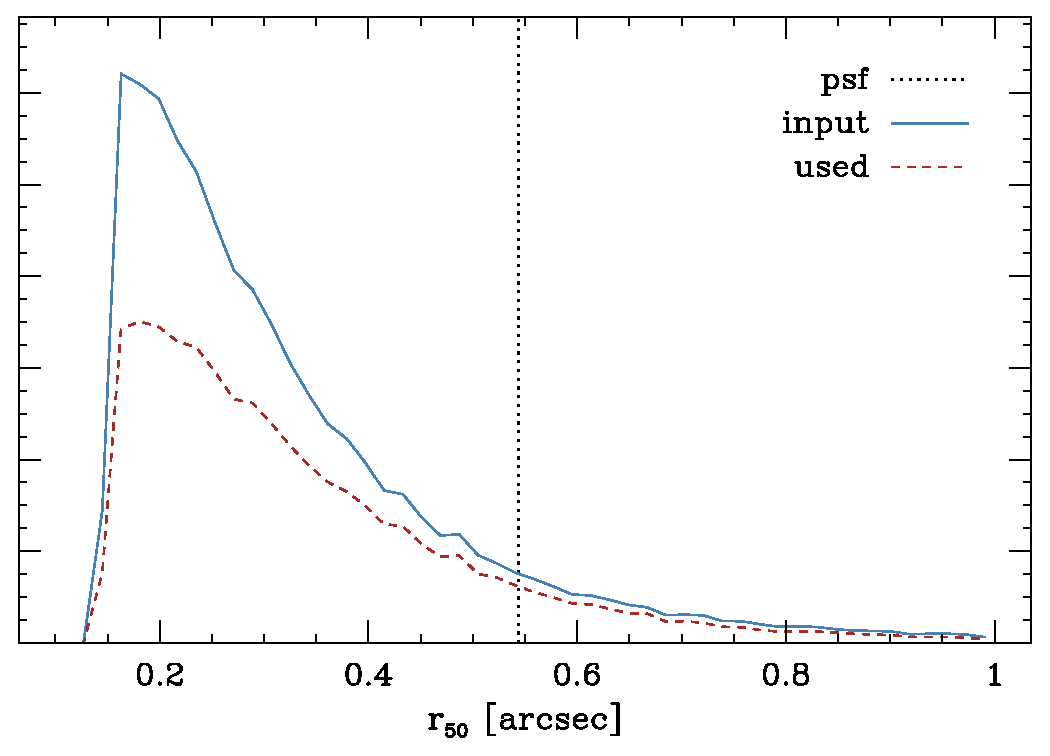
\includegraphics[width=\columnwidth]{run-bdj03mcal02-r50.eps}

    \caption{Distribution of half-light-radius \hlr\ in the parametric simulations.
        The solid line represents the distribution of input \hlr, drawn from fits
        to COSMOS data.  The dashed line represents the \hlr\ for objects that passed
		the initial $S/N > 5$ cut.  The \hlr\ of the PSF is shown as the vertical dotted
        line.}

\label{fig:psimhlrcompare}
\end{figure}

In figure \ref{fig:s2n} we show the distribution of \snr\ for the
parametric galaxies.  Shown are both the true input \snr\ and the
distrubtion of true \snr\ after applying a cut at {\it measured}
\snr$ > 5$.  The measured \snr\ is noisy and biased, being
based off a single-gaussian, resulting in a smooth rolloff
in the true \snr.

\begin{figure}
    \centering
    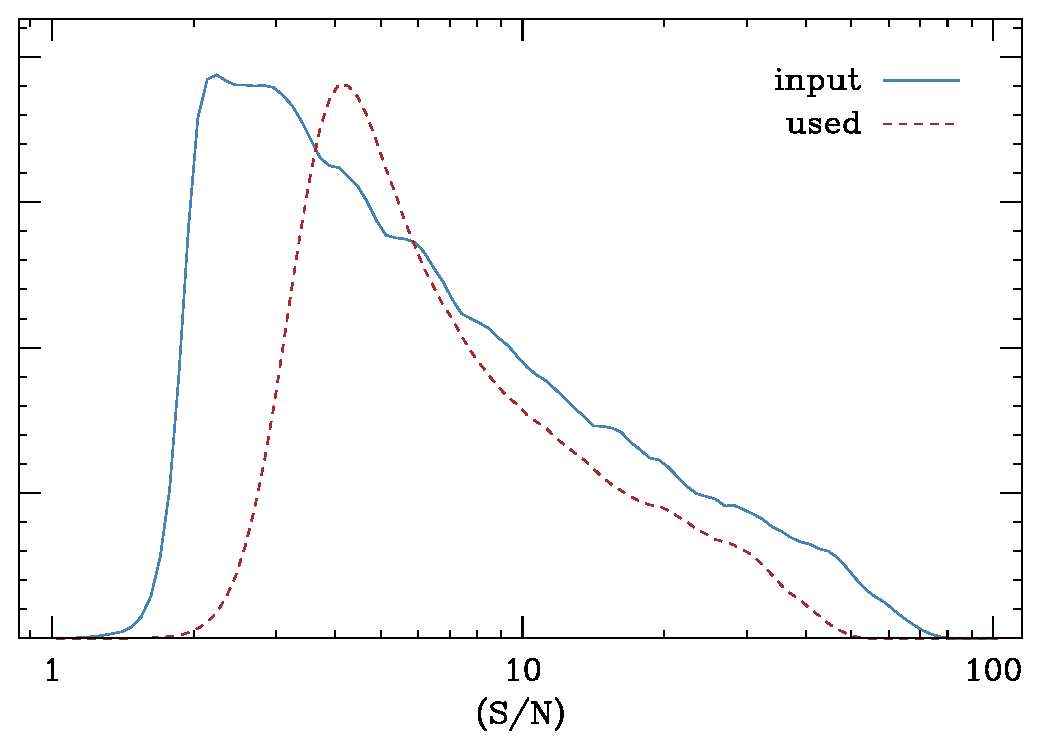
\includegraphics[width=\columnwidth]{run-bdj03mcal02-s2n.eps}

    \caption{Distribution of S/N in the parametric simulations. The
    solid curve represents the true input distribution, the dashed curve 
	represents the objects that passed the initial cut on {\it measured}
    \snr$ > 5$. The measured \snr\ was biased and noisy,
    resulting in a smooth selection on true \snr.}

\label{fig:s2n}
\end{figure}

\subsubsection{Simulated Stars}

Ideally, the ellipticity and \mcalR\ measured for stars should both be
consistent with zero in the mean, and thus not bias the ensemble shear
estimate.  In order to test the robustness of \mcal\ to stellar contamination,
we included $\sim$\nsimNstarperc\ stars in the \bdsim\ simulation.  The stars
were simply drawn as PSFs, with the same flux distribution as used for the
galaxies.  We refer to the simulation with stars as \bdstar; the
galaxies are identical to those in the \bdsim\ simulation, but stars
were then included in the analysis.

\begin{comment}
\subsubsection{Simulated Masking}

The Fourier transforms used to perform the \mcal\ convolutions cannot
accommodate missing data.  But in real data, ``bad pixels'' must be masked in
order to prevent biased measurements. For the FFTs, these masked pixels must be
replaced with some value that does not bias the shear recovery.

We created another set of simulations, called \bdmask, in which we masked
parts of the data in order to mimic certain effects in real images.  In order
simulate these effects realistically, we chose a sample of real bit mask planes
used in Dark Energy Survey shear analysis \citep{DESSVShear}.  These include
masking of bad pixels, bad columns, and other image artifacts.   We chose a random
random sample of \nmasks\ masks, after removing those for which a masked pixel
fell within 4 pixels of the image center.  An example image and mask are shown
in figure \ref{fig:mask}.

\begin{figure}
    \centering
    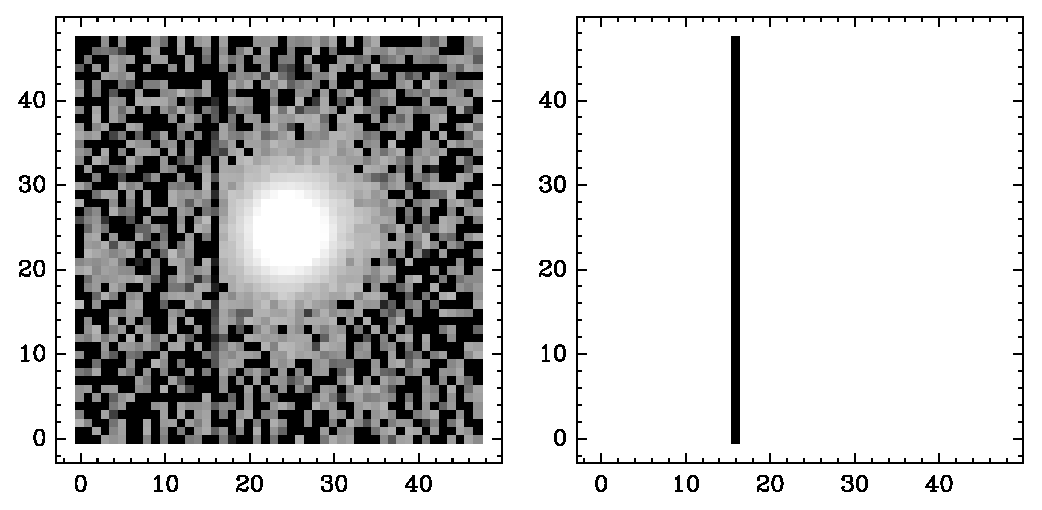
\includegraphics[width=\columnwidth]{DES2117+0126-bmask-021223.eps}

    \caption{Example DES image cutout and bitmask.  The vertical black stripe masks a
bad column. }

\label{fig:mask}
\end{figure}
\end{comment}

\subsubsection{Pre-selection} \label{sec:preselect}

We generated images with \snr\ down to $\sim 2$, as shown in figure
\ref{fig:s2n}, but we did not fit all these images to models.  In real data,
detections at these very low \snr\ can be spurious, so in practice a threshold
must be placed to produce what are considered reliable detections.  This type
of selection will result in a bias in the population of galaxy shapes, since
a round object has higher \snr\ than if it were sheared,
and galaxies oriented in the same direction as the PSF have higher \snr\
than objects otherwise oriented.  This effect will in turn bias
the shear recovery.

If this selection might occur before \mcal\ and object fitting, the corrections
for selection effects presented in \S \ref{sec:selection} cannot be used.

In order to test that we can recover the shear in the presence of this effect,
we applied a pre-selection at \snr$ > 5$, and \mcal\ was not run on the
galaxies that were removed.  We will apply further cuts on the \snr\ above this
threshold.  See \S \ref{sec:shear_recover} for details.


\subsection{Real Galaxy Simulations} \label{sec:cosmosim}

We designed a second set of simulations to mimic the ``real-galaxy'' constant
shear simulations used in GREAT3 challenge \citep{great3}, using galaxy images drawn
from 23.5 magnitude limited COSMOS data.  All galaxies in 1000 sub-fields were
given the same shear, ranging from 0.01 to 0.08, with random orientations.

We implemented two important changes as compared to GREAT3.  First, we oriented
the galaxies randomly, whereas in GREAT3 the galaxies were placed in pairs
rotated by 90 degrees, in order cancel shape noise.  Using paired galaxies has
the undesired effect of cancelling some biases that we want to explore
\citep{DESSVShear}.  Second, we used optical aberrations in the PSF designed to
match that seen in the Dark Energy Survey data\footnote{Aaron Roodman, private
communication}.  Similar to GREAT3, we varied the aberrations as Gaussian
random variables around a fiducial value. These root-mean-squared variations,
in units of waves in the Noll convention, are given in table \ref{tab:aberr}.
We used a Kolmogorov model for the atmospheric component, such that
the overall mean FWHM $\sim 0.9$ arcsec for 0.263 arcsec pixels.
For this configuration there are
significant variations in the PSF ellipticity, but relatively little net
ellipticity across the entire ensemble of realizations.  The code used to
generate these simulations began as a fork of the GREAT3 public code base, and
is freely available online\footnote{https://github.com/esheldon/egret}.

\begin{table}
    \centering
    \caption{Root-mean-squared variation for the aberrations in the optical model,
        in units of waves in the Noll convention, derived 
    from Dark Energy Survey data. \label{tab:aberr}}
    \begin{tabular}{ | l | l | }
        Zernike Component  & RMS Variation \\
        \hline
        Defocus & 0.13 \\
        Astigmatism in Y & 0.13 \\
        Astigmatism in X & 0.14 \\
        Coma in Y & 0.06 \\
        Coma in X & 0.06 \\
        Trefoil in Y & 0.05 \\
        Trefoil in X & 0.06 \\
        Spherical & 0.03 \\

    \end{tabular}
\end{table}

In figure \ref{fig:cosmos} we show the distribution of measured \snr\ for the
COSMOS simulations.  The mode of the distribution is significantly higher than that
of the parametric simulations, about 12 instead of 2.  Also shown is the
distribution of the half-light-radius \hlr, measured from the \sersic\ model
fits distributed with the 23.5 COSMOS catalog as part of the GREAT3 challenge,
including the selections applied for the simulation.  The mean \hlr\ for these
simulations is about \cosmosrdist, somewhat larger than the log-normal
\galrdist\ for the parametric simulations.


\begin{figure}
    \centering
    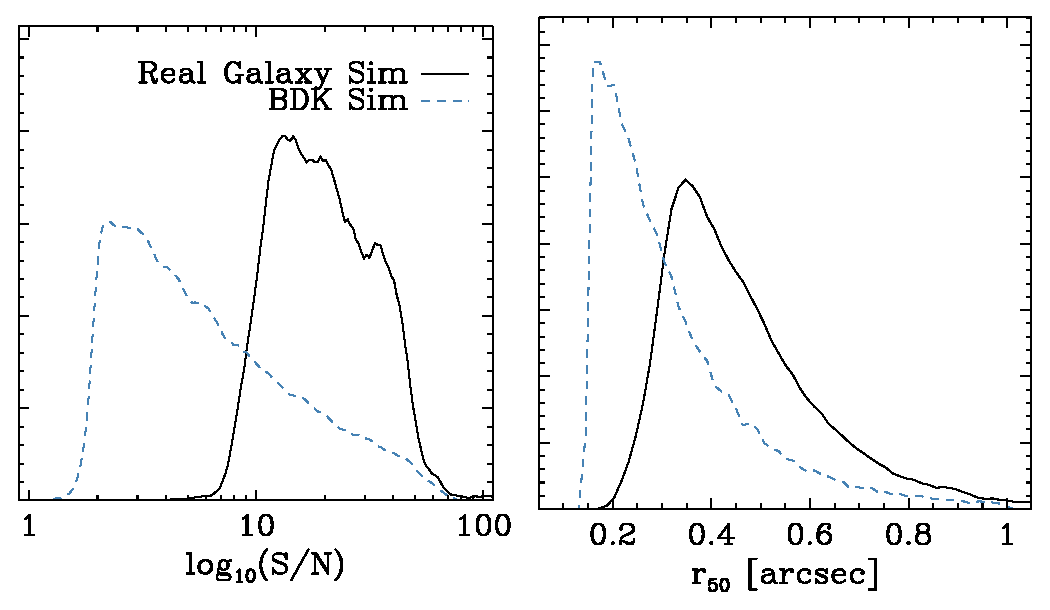
\includegraphics[width=\columnwidth]{mcal-v14s01-s2n-and-r50-with-nsim.eps}

    \caption{Distribution of properties in the COSMOS real galaxy simulations. The
    left panel contains the distribution of measured S/N, while the right panel contains
    the distribution of half-light-radius from the cosmos catalog for the input
    galaxies.  For comparison, the distributions for the BDK simulations
    are overplotted as dashed lines.}

\label{fig:cosmos}
\end{figure}

Note the parametric sims presented in \S \ref{sec:bdsim} used the fainter, and
smaller, 25.2 magnitude limited sample.  We thus do not expect the real galaxy
simulation to be more challenging than the parametric sim in every aspect. We
include it to directly address any special properties of real galaxies that may
not appear in our bulge+disk+knots simulation, and to test shear recovery using
a more realistic PSF.



\begin{table*}
    \centering

    \caption{Description of the image simulations.  For the \bdsim\
    simulations, the Bulge and Disk had independent ellipticities but the same
    half light radius \hlr.  The galaxy \hlr\ and flux were drawn from fits to the 25.2 mag.
    limited COSMOS sample.  Additionally, knots of ``star formation'' were added as
    point sources distributed as a random walk in the disk.  The \bdstar\
    simulation shared the same galaxy images with the \bdsim\ simulation, but
    with additional star images included.  For
    the \rgsim\ simulation, real COSMOS images were used for the galaxies. For
    the PSF, a  Kolmogorov atmospheric turbulence model was used, 
    plus contributions from an optical model matched to DES; the mean PSF size
    was approximately 0.9 arcsec. The PSF ellipticity is given in the "reduced
    shear" convention.
    \label{tab:sims}}

    %\scriptsize
    \begin{tabular}{ | l | c | c | c | c | c | c | c | c | }
        Sim          & Galaxy Model      & Size \& Flux   & PSF Model   & PSF FWHM        & PSF shape     & Shear & \# Galaxies    & \# Stars     \\
                     &                   &             &             & [arcsec]        &               &       &               &              \\
        \hline
        \rgsim       & \cosmosname       & \cosmosname & Kolm./Opt.  & \psfrdist/Opt.  & Optical       &  Variable & \nsimNgal     & None            \\
        \bdsim       & Bulge+Disk+Knots  & \galrdist   & Moffat      & \psfrdist       & \nsimPSFShape &  \nsimShear & \nsimNgalBD & None            \\
        \bdstar      & Bulge+Disk+Knots  & \galrdist   & Moffat      & \psfrdist       & \nsimPSFShape &  \nsimShear & \nsimNgalBD & \nsimNStar       \\
    \end{tabular}
\end{table*}

\section{Model Fitting and Metacalibration Operations} \label{sec:modelfit}

We fit the images with a single Gaussian model using the \ngmix\
code\footnote{https://github.com/esheldon/ngmix}.  To perform the fit we used an
implementation of the ``adaptive moments'' algorithm originally presented in
\cite{bern02}.   We applied no PSF correction.  We expect this estimator to
respond poorly to a shear, but we will measure this weak response using \mcal.

Rather than attempt to correct for psf anisotropy using \mcal\ ``psf response''
as was done in \cite{HuffMcal}, we instead reconvolved by a symmetrized version
of the PSF. We created this PSF by adding the PSF image to itself, rotated by
90, 120, and 180 degrees.  This averaging can result in a PSF that is smaller
in some dimensions than the original, so we further dilated this symmetrized
PSF.  The dilation factor was taken to be $1+2*\delta$, where
\begin{align}
    %\delta = \frac{E}{0.5 (<x^2> + <y^2>)}
    \delta = \frac{E}{T/2}
\end{align}
Here $E$ is the maximum eigenvalue from the covariance matrix of the best-fit
Gaussian. This we divide by half the trace $T$, which is the mean extent of the
object.  For a purely elliptical PSF, a factor of $1+\delta$ would be
sufficient; we conservatively increase the factor to $1+2\delta$ in case the
Gaussian fit does not completely capture the asymmetries of the true PSF.

All \mcal\ image operations were performed using the \texttt{metacal} module
from \ngmix, which in turn uses GALSIM to perform most image manipulations.
Before fitting, we added a noise field designed to correct for correlated
noise, as discussed in \S \ref{sec:fixnoise}


\section{Results} \label{sec:results}


\subsection{\Mcal\ Responses}

In figure \ref{fig:Rstars} we show the measured \mcal\ responses for
the \bdsim\  simulations.  Also shown is the response with stars included.
The distrubution of \mcalR\ is quite symmetric in the absence of stellar
contamination.  We will discuss the affect of stars in \S \ref{sec:stars}.

\begin{figure}
    \centering
    %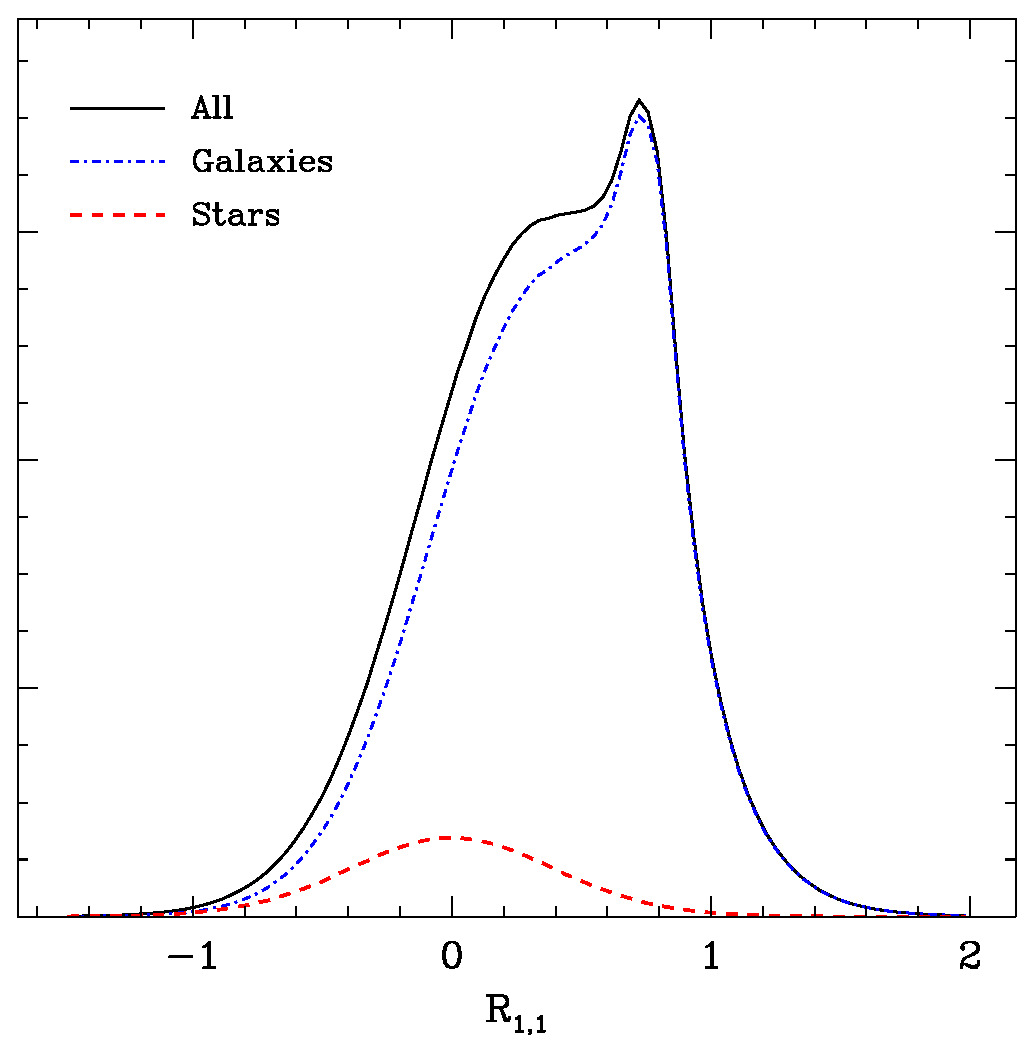
\includegraphics[width=\columnwidth]{R-bd29-bd29stars.eps}
    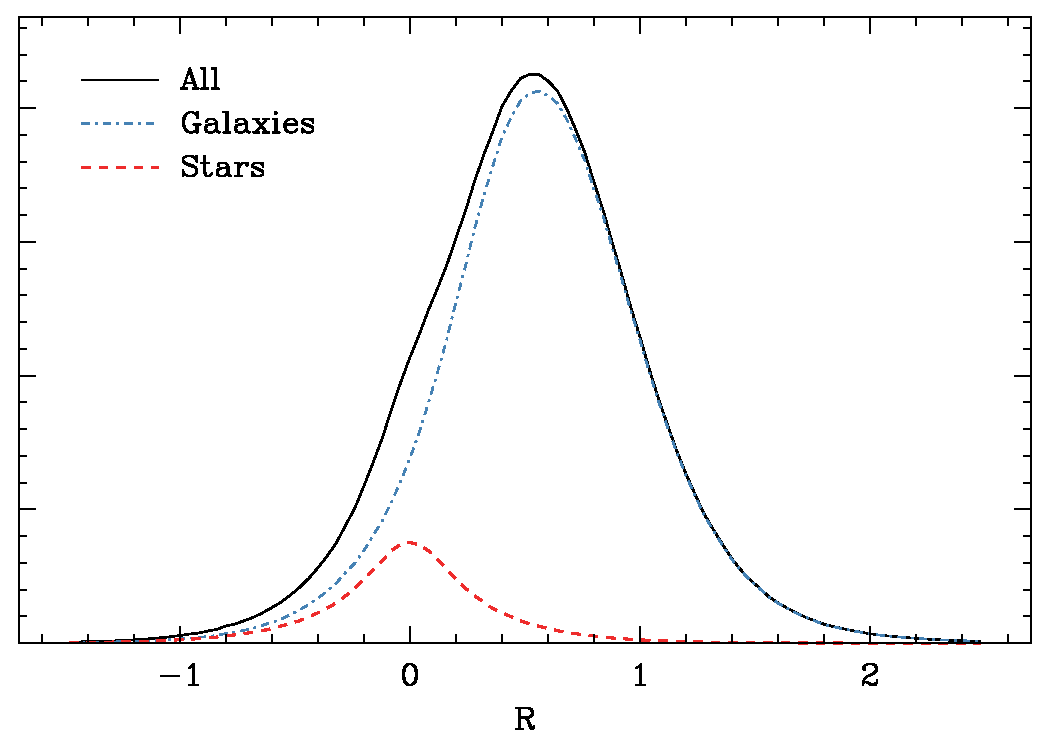
\includegraphics[width=\columnwidth]{R-bdj03-bdj03stars.eps}

    \caption{Distribution of \mcal\ responses for galaxies and stars in
    the \bdstar\ simulation.  Stars have mean response close to zero,
    and thus do not bias the overall shear calibration.}

\label{fig:Rstars}
\end{figure}



\subsection{Shear Recovery} \label{sec:shear_recover}


In table \ref{tab:results} we show results for shear recovery in each of our
simulations.  As was discussed in \S \ref{sec:preselect}, we applied a
pre-selection to the \bdsim\ simulation at \snr$ > 5$, which imposes a
selection bias.  We thus placed cuts at higher \snr\ than this threshold, so
that the corrections for selection effects presented in \S \ref{sec:selection}
could be used accurately.  In this table we show results for \snr$ > 10$.  
For the \rgsim\ simulation we did not apply a pre-selection.

Using \mcal\ we found no significant multiplicative or additive biases in any
case.  Without applying the \mcal\ responses, the multiplicative bias $m$ was of
order 50\% for all simulations.

\begin{table*}
    \centering
    \caption{\Mcal\ results for each image simulation described in
        \S \ref{sec:sims} and table \ref{tab:sims}.  For each simulation,
        a cut was placed at \snr$ > 10$, and corrections were applied
        for selection effects (see table \ref{tab:results_sel} for more
        results on selections).  A single Gaussian was fit
    to the observed object, with no PSF correction applied.
    No multiplicative or additive bias was detected in any case. 
    Stellar contamination at the level of \nsimNstarperc\ increases
    the noise in the recovered shear by \starnoiseincrease\ but does not introduce 
    a significant bias.  
    \label{tab:results}}
    \begin{tabular}{ |l|  c|c|c|  c|c|c|}
        \hline
        Sim    & $m$               & $c_1$            & $c_2$ \\
               & $[10^{-3}]$       & $[10^{-5}]$      & $[10^{-5}]$ \\
        \hline
        %\rgsim & $+0.22 \pm 0.58$  & $+0.26 \pm 0.29$ & $+0.22 \pm 0.29$ \\
        \rgsim & $0.22 \pm 0.58$  & $2.6 \pm 2.9$    & $2.2 \pm 2.9$ \\
        \bdsim & $0.03 \pm 0.31$  & -                & $-0.15 \pm 0.62$ \\
        \bdstar& $0.01 \pm 0.32$  & -                & $-0.08 \pm 0.63$
    \end{tabular}
\end{table*}

%        \bdmask& $-496$      & $+0.09 \pm 0.10$ & $ 15.07 \pm 0.10$ & $-0.60 \pm 0.46$  & $-0.17 \pm 0.23$ & $0.73 \pm 0.23$  \\


\subsubsection{Results with Selection Effects}

In table \ref{tab:results_sel}, we show the results for different \snr\
threshold cuts in the \bdsim\ simulations.  We show the recovered bias with and
without corrections for selection effects.  These results are also shown
graphically in figures \ref{fig:s2nthresh} and \ref{fig:s2nthresh_nocorr}.  The
cuts were all placed above the pre-selection at \snr$ > 5$, to guarantee the
validity of the corrections.

We found a significant multiplicative selection bias in each case.  These
biases are well above the requirements for current and future experiments, and
thus must be corrected.  We find \mcal\ corrects these biases to within the
requirements of future surveys in all cases.  We did not find any 
additive selection biases, which suggests our procedure of reconvolving by
a symmetrized PSFs is working as expected.

\begin{table*}
    \centering
    \caption{\Mcal\ results for the \bdsim\ simulation with various
        cuts on \snr.   Results are shown with and without corrections
        for selection effects.
    \label{tab:results_sel}}
    \begin{tabular}{ |l| c|c|  c|c|}
        \hline
        & \multicolumn{2}{c}{Uncorrected for Selection}                      & \multicolumn{2}{c}{Corrected for Selection} \\
        Selection                   & $m$             & $c$            & $m$               & $c$  \\
                                    & $[10^{-3}]$     & $[10^{-5}]$    & $[10^{-3}]$       & $[10^{-5}]$ \\
        \hline
$\mbox{\snr} > 7 $ & $+15.55 \pm 0.34$ & $+0.80 \pm 0.68$ & $+0.55 \pm 0.34$ & $+0.79 \pm 0.67$ \\
$\mbox{\snr} > 10 $ & $+3.78 \pm 0.31$ & $-0.15 \pm 0.62$ & $+0.03 \pm 0.31$ & $-0.15 \pm 0.62$ \\
$\mbox{\snr} > 13 $ & $-1.46 \pm 0.31$ & $+0.27 \pm 0.63$ & $+0.03 \pm 0.31$ & $+0.27 \pm 0.63$ \\
$\mbox{\snr} > 16 $ & $-4.58 \pm 0.33$ & $+0.44 \pm 0.67$ & $+0.26 \pm 0.34$ & $+0.44 \pm 0.67$ \\
$\mbox{\snr} > 19 $ & $-8.33 \pm 0.36$ & $+0.17 \pm 0.73$ & $+0.05 \pm 0.37$ & $+0.18 \pm 0.73$ \\
    \end{tabular}
\end{table*}


\begin{comment}
\begin{table*}
    \centering
    \caption{\Mcal\ results for the \bdsim\ simulation with various
        cuts on \snr.   Results are shown with and without corrections
        for selection effects.
    \label{tab:results_sel}}
    \begin{tabular}{ |l| |c| c|c|c|  c|c|c|}
        \hline
        & & \multicolumn{3}{c}{Uncorrected for Selection}                      & \multicolumn{3}{c}{Corrected for Selection} \\
        Selection                   & Fraction Kept & $m$             & $c_1$            & $c_2$            & $m$               & $c_1$            & $c_2$ \\
                                    &               & $[10^{-3}]$      & $[10^{-4}]$      & $[10^{-4}]$      & $[10^{-3}]$       & $[10^{-4}]$      & $[10^{-4}]$ \\
        \hline
        $\mbox{\snr} > 0$           & 1.00          & -                & -                & -                & $-0.91 \pm 0.19$  & $-0.04 \pm 0.09$ & $+0.17 \pm 0.09$  \\
        $\mbox{\snr} > 7$           & 0.83          & $+2.53 \pm 0.19$ & $-0.05 \pm 0.10$ & $0.93 \pm 0.10$  & $-0.15 \pm 0.19$  & $-0.05 \pm 0.10$ & $+0.17 \pm 0.10$  \\
        $\mbox{\snr} > 10$          & 0.60          & $+3.48 \pm 0.20$ & $-0.00 \pm 0.10$ & $0.81 \pm 0.10$  & $-0.10 \pm 0.20$  & $-0.00 \pm 0.10$ & $+0.15 \pm 0.10$  \\
        $\mbox{\snr} > 13$          & 0.46          & $+2.61 \pm 0.20$ & $+0.04 \pm 0.10$ & $0.58 \pm 0.10$  & $-0.09 \pm 0.20$  & $+0.04 \pm 0.10$ & $+0.13 \pm 0.10$  \\
        $\mbox{\snr} > 16$          & 0.39          & $+1.85 \pm 0.21$ & $+0.07 \pm 0.11$ & $0.49 \pm 0.11$  & $-0.04 \pm 0.21$  & $+0.07 \pm 0.11$ & $+0.14 \pm 0.11$  \\
        $\mbox{\snr} > 19$          & 0.33          & $+0.98 \pm 0.22$ & $+0.03 \pm 0.11$ & $0.42 \pm 0.11$  & $-0.23 \pm 0.22$  & $+0.03 \pm 0.11$ & $+0.12 \pm 0.11$  \\

        \hline

        $\mbox{\snr} \in [ 7,  16]$ & 0.44          & $+3.68 \pm 0.38$ & $-0.29 \pm 0.19$ & $1.70 \pm 0.19$  & $-0.37 \pm 0.38$  & $-0.29 \pm 0.19$ & $+0.22 \pm 0.19$  \\
        $\mbox{\snr} \in [16,  37]$ & 0.22          & $+4.55 \pm 0.33$ & $+0.12 \pm 0.17$ & $0.70 \pm 0.17$  & $-0.41 \pm 0.33$  & $+0.12 \pm 0.17$ & $+0.21 \pm 0.17$  \\
        $\mbox{\snr} \in [37,  87]$ & 0.10          & $+0.21 \pm 0.37$ & $-0.27 \pm 0.19$ & $0.04 \pm 0.19$  & $+0.14 \pm 0.37$  & $-0.13 \pm 0.19$ & $-0.17 \pm 0.19$  \\
        $\mbox{\snr} \in [87, 200]$ & 0.04          & $-2.00 \pm 0.52$ & $-0.04 \pm 0.26$ & $0.81 \pm 0.26$  & $+0.22 \pm 0.52$  & $-0.04 \pm 0.26$ & $+0.61 \pm 0.26$  \\

        %$\mbox{\snr} \in [7, 10.84]$      & 0.27     & $-0.37 \pm 0.55$ & $-0.38 \pm 0.27$ & $1.78 \pm 0.27$  & $-0.11 \pm 0.55$  & $-0.38 \pm 0.27$ & $0.27 \pm 0.27$  \\
        %$\mbox{\snr} \in [10.84, 22.73]$  & 0.27     & $+7.44 \pm 0.37$ & $-0.03 \pm 0.18$ & $1.16 \pm 0.18$  & $-0.41 \pm 0.37$  & $-0.03 \pm 0.18$ & $0.09 \pm 0.18$  \\
        %$\mbox{\snr} > 22.73$          & 0.27     & $+0.47 \pm 0.23$ & $+0.05 \pm 0.12$ & $0.46 \pm 0.12$  & $-0.02 \pm 0.23$  & $+0.05 \pm 0.12$ & $0.20 \pm 0.12$  \\


    \end{tabular}
\end{table*}
\end{comment}


\begin{figure}
    \centering
    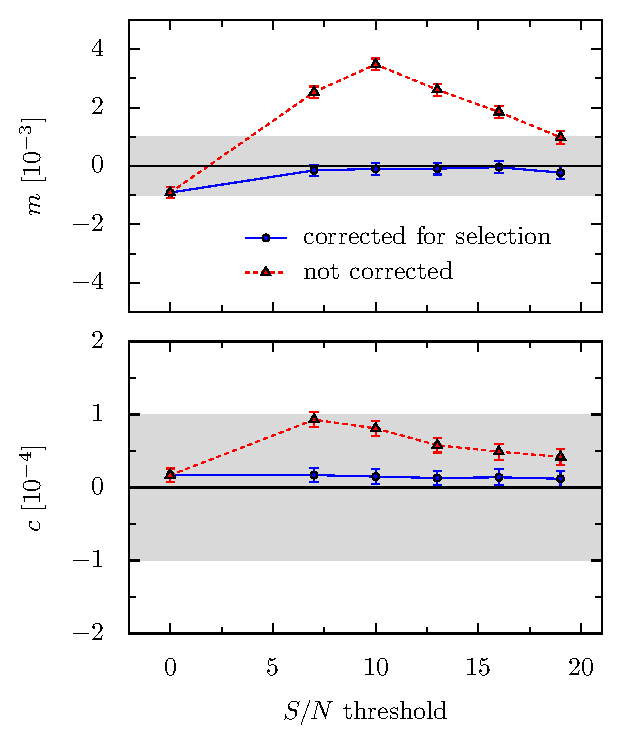
\includegraphics[width=\columnwidth]{mc-select-bias-thresh.eps}

    \caption{Multiplicative (upper panel) and
		additive bias (lower panel) in the \bdsim\ simulation after applying
        threshold selections in \snr.   
        The filled grey region represents the target accuracy. } 

\label{fig:s2nthresh}
\end{figure}


\begin{figure}
    \centering
    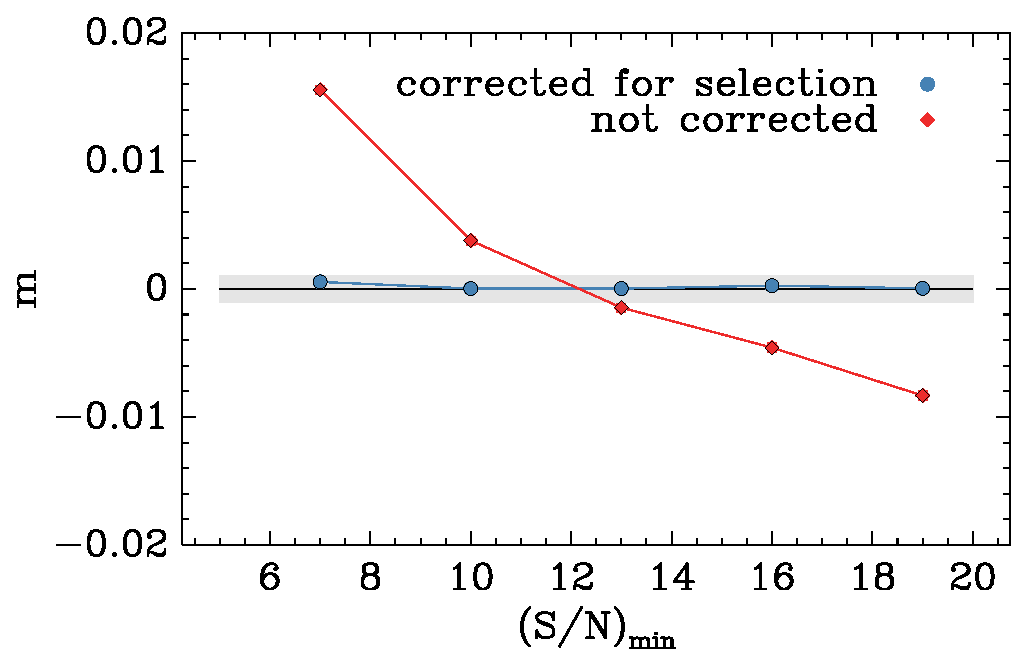
\includegraphics[width=\columnwidth]{mc-select-bias-thresh-with-nocorr.eps}

    \caption{Multiplicative in the \bdsim\ simulation after applying
        threshold selections in \snr.  The bias without correction for
        selection effects is represented as as red diamonds. The bias after
        correction for selection effects is represented as blue circles.  
        The filled grey region represents the target accuracy. } 

\label{fig:s2nthresh_nocorr}
\end{figure}


%\begin{figure}
%    \centering
%    %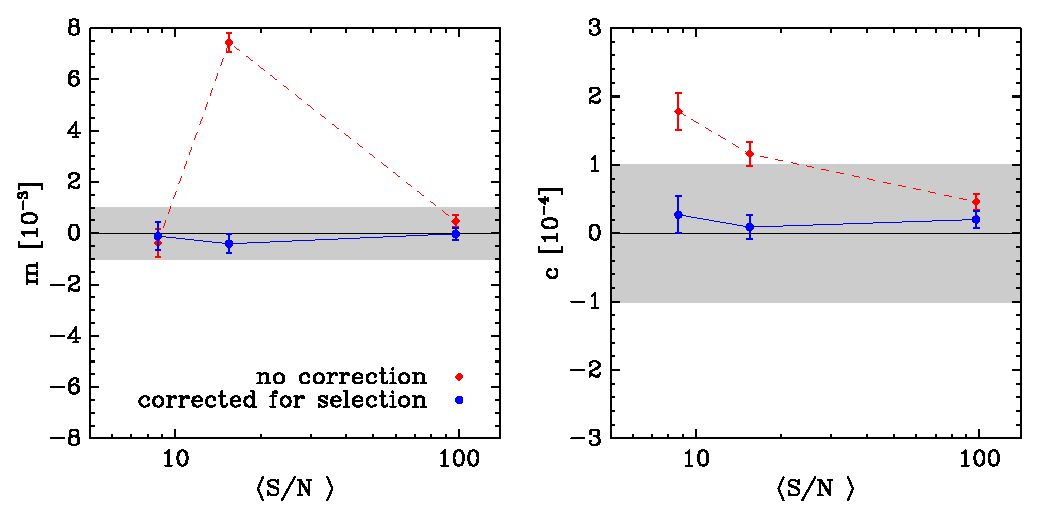
\includegraphics[width=0.9\textwidth]{mc-select-bias-range.eps}
%    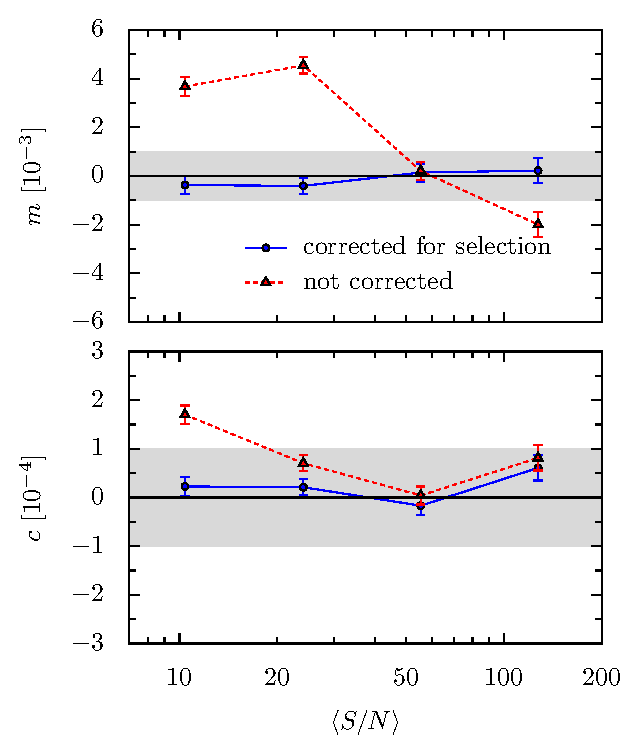
\includegraphics[width=\columnwidth]{mc-select-bias-range-pyx.eps}

%    \caption{Bias in the \bdsim\ simulation after applying
%        range selections in \snr.  The left panel represents
%        the multiplicative bias $m$ and the right panel the additive
%        bias $c$.  The bias without correction for
%        selection effects is represented as as red diamonds. The bias after
%        correction for selection effects is represented as blue circles.  } 

%\label{fig:s2nrange}
%\end{figure}



\subsubsection{Results with Stellar Contamination} \label{sec:stars}

Results including \nsimNstarperc\ stars in the \bdstar\ simulation are shown in
table \ref{tab:results}. We did not detect any additional bias due to including
stars. The noise did, however, increase by \starnoiseincrease.

%As indicated in table \ref{tab:sims}, for the \bdstar\  type simulations, we
%included an additional \nsimNStar\ stellar objects, \nsimNstarperc, drawn
%simply as a PSF with noise added.  The galaxy images were the same as used in
%the \bdsim\ simulation.  The results are shown in table \ref{tab:results}.  

\Mcal\ is robust to stellar contamination if the PSF is well
characterized.  Images consistent with a PSF will not, in the mean, respond to the shear
applied during the \mcal\ process.  Measurement on stars also yields zero average shape, as
long as the PSF correction is sufficiently accurate: our use of a symmetrized
PSF (see \S \ref{sec:modelfit}) appears to be sufficient in this case.
In figure \ref{fig:Rstars} we show the measured response \mcalR\ for stars and
galaxies.  Indeed we see that, for stars, the \mcalR\ is noisy but consistent
with zero.

If the additional variance is tolerable, it may be useful to include stars in a
shear analysis if the PSF is sufficiently well known.  Attempting to remove
faint stars from a sample is a noisy procedure, likely to induce selection
effects.  These can be controlled using the corrections derived in \S
\ref{sec:selection}, but only if the selection is also repeated based on
quantities measured on sheared images, so the corrections can be calculated.
If the selection must be performed outside of the \mcal\ process, it may be
better to avoid it altogether.

For accurate interpretation of the signal, it is still important that any
redshift estimates for the stars are consistent with zero, in the mean. It
is also important to weight by the \mcal\ response terms in order to
get the correct mean; see \S \ref{sec:weighting} for more discussion
of weighted means.



\begin{comment}
.  We can
rewrite equation \ref{eq:basicestimator} as
\begin{align}
    \langle \gamma \rangle &= \frac{ \sum E }{\sum \mbox{\mcalR}} = \frac{ \sum \mbox{\mcalR}^{true} \gamma }{\sum \mbox{\mcalR}},
\end{align}
which would look like a weighted average if the measured \mcalR\ were equal to
the true response $\mbox{\mcalR}^{true}$.  The measured \mcalR\ could be used
to weight the redshift estimates as well, although one must be careful as the
\mcalR\ are not strictly positive.
\end{comment}

\begin{comment}
\subsubsection{Results with Masking Effects} \label{sec:masking}

Here we discuss the results for the \bdmask\ simulation, introduced in \S
\ref{sec:bdsim}.  In this simulation, we mocked up masking of ``bad'' pixels,
columns, and other artifacts using masks drawn from real DES data.

As a baseline extreme case, we replaced the masked pixels simply with noise.
This resulted in significant calibration bias.

%In order to perform the Fourier transforms used for the \mcal\ convolutions, we
%must replace any missing data with an appropriate value.  For example, some
%pixels may be marked as ``bad'', and masked in the data reduction pipeline.  In
%particular we wish to avoid any artifacts in the transformed images that would
%mimic an additional ``response'' to the applied \mcal\ shear.

A better alternative is to replace the missing data with the result of our
model fit.  Since we used a Gaussian model for both PSF and Galaxy, which is a
poor representation of the data, we consider this a worst case scenario as a
model replacement. 

The results using the model replacement method are shown in table
\ref{tab:results} for the \bdmask\ simulation.  The measured bias did not
change significantly compared to the measurements on the independent \bdsim\
simulation.

\end{comment}


\begin{comment}
There are two main types of selection: detection effects and ordinary selection
effects.  Detection effects occur when placing a detection threshold on a
quantity that correlates with galaxy shape. One example is \snr: cutting to
objects greater than some value of \snr\ will preferentially remove galaxies
with higher ellipticity, and thus reduce the inferred shear.  Ordinary
selection on an initially unbiased detected sample can induce additional bias
via the same mechanism.

Determining detection effects may require prior information about the
properties of the galaxies in the sample, including those galaxies that do not
exceed the detection threshold.  Ordinary selection effects can in principle be
determined from the noisy data, without prior information. If the initial
detections were unbiased, one can examine how shearing galaxies changes their
probability of selection near the threshold.  A similar technique can be
applied even in the presence of a biased detection if the additional selection
is relatively stringent, so that the original detection cut can be ignored,

To test selection effects, we made a series of cuts on S/N in the \bdsim\
simulation.  We used the ``round'' \snr\ definition in order to avoid the first
order effect \citep{DESSVShear}.  We found the magnitude of the multiplicative
bias increased monotonically with the cut on \snr, reaching a bias of $\sim
-2.5 \times 10^{-3}$ for $S/N > 20$.  This bias is larger than the requirements
for future surveys.

The detection bias could potentially be even larger than what we found, since
the cut would be applied to a distribution of intrinsic \snr\ that ha
an approximately power law shape, rather than one with a cutoff, as we had in
our simulations. We will explore how to mitigate these important selection
effects in a future work.
\end{comment}

\begin{comment}
As indicated in table \ref{tab:selresults},
these cuts lead to a monotonic change in the recovered shear, with a few
tenths of a percent bias for a $S/N > 20$ cut.

\begin{table*}
    \centering
    \caption{\Mcal\ results when applying selections on the signal-to-noise ratio (S/N) to the \bdsim\ simulations. Selections
    were applied to an initially unbiased sample; i.e. no {\em detection}
    bias was present in the sample. \label{tab:selresults}}
    \begin{tabular}{ |l| r|r|r|  r|r|r|}
        \hline
        & \multicolumn{3}{c}{Uncorrected for Selection} & \multicolumn{3}{c}{Corrected for Selection} \\
        Selection & $m \times 10{^3} $ & $c_1 \times 10^4$ & $c_2 \times 10^4$ & $m \times 10^{3}$ & $c_1 \times 10^4$ & $c_2 \times 10^4$ \\
        \hline
        %$(S/N) > 5$    & $3.0 \pm 4.4$ & $-0.3 \pm 0.2$ & $0.2 \pm 0.2$ & $3.3 \pm 4.4$ & $-0.3 \pm 0.2$ & $0.2 \pm 0.2$  \\
        $(S/N) > 7.5$  & $-0.7 \pm 0.4$ & $-0.3 \pm 0.2$ & $0.2 \pm 0.2$ & $-0.6 \pm 0.4$ & $-0.3 \pm 0.2$ & $0.2 \pm 0.2$  \\
        $(S/N) > 10$   & $-1.5 \pm 0.5$ & $-0.3 \pm 0.2$ & $0.2 \pm 0.2$ & $-1.0 \pm 0.5$ & $-0.3 \pm 0.2$ & $0.2 \pm 0.2$  \\
        $(S/N) > 15$   & $-2.3 \pm 0.5$ & $0.0 \pm 0.3$ & $0.0 \pm 0.3$ & $-0.9 \pm 0.5$ & $0.0 \pm 0.3$ & $0.0 \pm 0.3$  \\
        $(S/N) > 20$   & $-2.7 \pm 0.6$ & $-0.3 \pm 0.3$ & $-0.2\pm 0.3$ & $-0.9 \pm 0.6$ & $-0.3 \pm 0.3$ & $-0.2 \pm 0.3$  \\
    \end{tabular}
\end{table*}

We implemented a simple correction based on our \mcal\ measurements.  We
sheared the population of ellipticities with a fake shear using the measured
responses \mcalR, and estimated the shear using our \mcal\ mechanism before and
after selection.  We then used the ratio of these numbers as a correction
factor.  We sow the results in table \ref{tab:selresults} in the ``Corrected
for Selection'' column.  This simple correction reduced the bias approximately
$10^{-3}$ in all cases.

In real data, a simple correction scheme like the above will probably require
prior information.  One approach would be to take deep imaging data and add
noise such that the distribution of $S/N$ for the galaxy sample is similar to a
shallower data set.  The noisy ellipticity measurements could then be sheared
artificially and selected as above to derive a correction.  Multiple noise
realizations could be used to increase the precision of the correction.
\end{comment}

\begin{comment}
\section{Bias in GREAT3 Simulations}

Relatively little bias was seen by \cite{HuffMcal} using the GREAT3 simulations
\citep{great3}.  We checked that our code used to perform the metacal
procedures gives identical results to that used in \cite{HuffMcal}, so this is
most likely not a software error.  We
suspect that the higher S/N of the GREAT3 simulations, and better modeling used
in \cite{HuffMcal} resulted in reduced bias.

The correlated noise effect scales with the square of the noise, and the
simulations used for GREAT3 contain significantly higher S/N galaxies than the
simulations used in this work.  Indeed, we found the correlated noise was still
detectable in simulations we ran with similar properties to GREAT3, but with
correlated noise bias at the 1-2\% level rather than the 12\% we saw in our
\rgsim\ simulations.  We also ran the re-gaussianization code on our
simulations, and did see a bias, but about a factor of two lower than we saw
for our intentionally bad Gaussian PSF and Galaxy models.

Another important difference between the GREAT3 sims and our sims is that
GREAT3 galaxies were generated in pairs, rotated by 90 degrees with respect to
a one another, in order to cancel shape noise.  However, we ran one of our
simulations in such a configuration and saw the same level of correlated noise
bias.  This is not surprising; the correlated noise effect adds coherently to
the response, and should not cancel due to such imposed symmetries in the
underlying galaxy population.
\end{comment}

\section*{Acknowledgments}

ES is supported by DOE grant DE-AC02-98CH10886.

We thank Aaron Roodman for providing the variation of the optical aberrations
measured in DES data.  Thanks to Mike Jarvis and Rachel Mandelbaum for guidance
on use of the GALSIM package, especially concerning use of the isotropization
and whitening features.  Thanks to Gary Bernstein for pointing out a simpler
form for the response for 2-point functions.


\appendix

\section{Additional Correction Methods} \label{sec:altcorr}

\subsection{Correction using GALSIM Methods}

With guidance from the GALSIM developers, we attempted to use the GALSIM noise
isotropization and whitening functionality to correct the correlated noise.
Isotropization enforces four fold symmetry, introducing minimal extra noise,
while whitening completely whitens the image, introducing significant extra
noise.  However, neither of these methods improved the shear recovery in our
simulations.  It may be that some aspects of the \mcal\ procedure invalidate
the assumptions behind these correction methods.


\subsection{Detrending the Correlated Noise Bias} \label{sec:detrend}

We expect the bias in \mcalR\ due to correlated noise to scale with the square
of the noise in the image $n^2$ (see \S \ref{sec:scaling}).  We can add a small
amount of noise to the image such that $n \rightarrow n + \Delta n$.  If we
then run the new image through the \mcal\ process, we can measure
$R^{\mathrm{before}}$, a response that will include correlated noise effects.
We can write this observed response as
\begin{align}\label{eq:Rbefore}
    R_o^{\mathrm{before}} &= R + A (n + \Delta n)^2 \nonumber \\
       &\simeq R + A n^2 + 2 A n \Delta n
\end{align}
%&\simeq R + A n^2 + \frac{\partial (An^2)}{\partial n} \Delta n + ... \nonumber \\
where we have dropped terms of order $(\Delta n)^2$ and higher.  In equation
\ref{eq:Rbefore}, \mcalR\ is the response at noise $n+\Delta n$ in the absence
of correlated noise.  

We can also add identical noise {\em after} the original image  has been run
through \mcal, and measure $R^{\mathrm{after}}$.  The response when adding
noise after \mcal\ does not suffer any additional bias due to correlated noise:
\begin{align}
    R_o^{\mathrm{after}} &= R + A n^2.
\end{align}
The difference between these responses is then 
\begin{align}
    \Delta R &\equiv R_o^{\mathrm{before}} - R_o^{\mathrm{after}}  \nonumber \\
             &\simeq 2 A n \Delta n.
\end{align}

We propose the following procedure to correct for correlated noise:
\begin{enumerate}
    \item Calculate $\Delta R$ for a series of noise offsets $\Delta n$.
    \item Average $\Delta R$ over all objects for each noise offset.
    \item Perform a linear fit to $\Delta R$ vs. $2 n \Delta n$ to find the 
        coefficient $A$.
    \item Apply a mean correction for correlated noise given by
        \begin{align}
            \mbox{\mcalRnoise} & \simeq A n^2.
        \end{align}
        with a similar correction for \mcalRpsf.
\end{enumerate}
If the noise varies between observations, we can apply a 
correction based on the mean variance $A
\langle n^2 \rangle$.

\subsubsection{Measurements of the \detrend\ Parameters}

For the \detrend\ method, we measured $\Delta R$ vs $2 n \Delta n$ to find the
coefficient $A$.  In figure \ref{fig:detrend}, we show this fit for the \rgsim\
simulation.  The trend is well-fit by a linear model, as expected, with a slope
$A \simeq $\Aslope, implying a correction $A n^2 \simeq$ \Rcorr\ for this
simulation.

\begin{figure}
    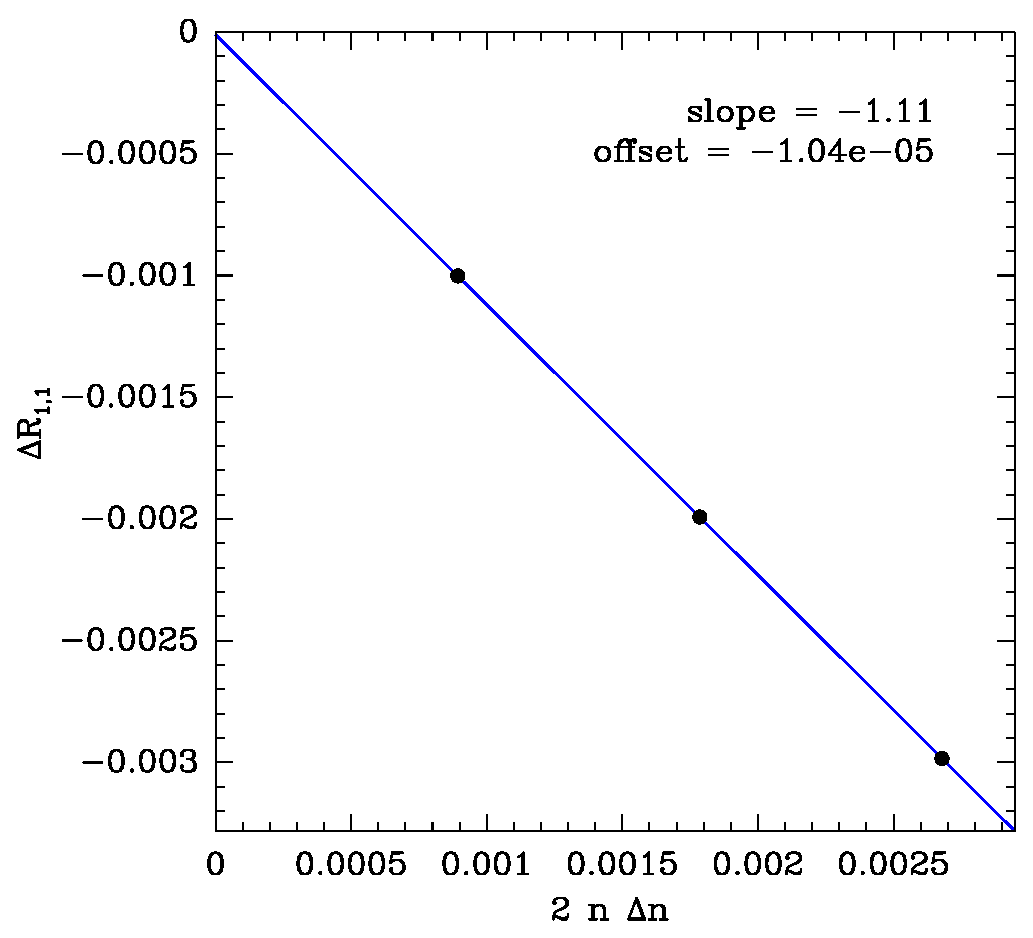
\includegraphics[width=\columnwidth]{mcal-v14s01-Rnoise-detrend-R11.eps}

    \caption{Trend of $\Delta R_{1,1}$ with $2 n \Delta n$ for the
        real galaxy simulation.   $n$ is the
    original noise level and $\Delta n$ is the additional noise added.  The
    trend is linear as predicted.}

\label{fig:detrend}
\end{figure}




\subsubsection{Using a Random Subset To Calculate \Detrend\ Corrections}

Measuring the \detrend\ parameters requires extra computations, at least a
factor of three to fit the linear parameters given in \S \ref{sec:detrend}, and
a factor of four if an additional point is used to check for possible
non-linearity. These extra computations could be expensive for large surveys.  

However, the \detrend\ parameters are more precisely measured than the shear
itself.  Here we explore the precision of the recovered shear using smaller
subsets of the object catalog to measure the \detrend\ parameters, and
applying the corrections to the full sample.  In Table \ref{tab:subsets}
we show the shear recovery parameters for various subset sizes, for the
\bdsim\ simulation described in \S \ref{sec:results}

\begin{table*}
    \centering
    \caption{Additional variance in the recovered shear 
        using different sized subsets to
        estimate the detrending corrections.  Values were obtained
        from 100 bootstrap samples. \label{tab:subsets}}
    \begin{tabular}{| c | c |}
        Subset Size & Extra Error \\
        \hline
        1\% & 4.4\% \\
        5\% & 0.8\% \\
        10\% & 0.3\% \\
    \end{tabular}
\end{table*}
%        1\% & 30\% \\
%        5\% & 13\% \\
%        10\% & 8\% \\


We find that a relatively small sample can be used to determine the correlated
noise correction.  Calculating the detrending terms for 10\% of the sample
leads to only 0.3\% extra variance in the recovered shear, and using 1\% of
galaxies leads to only 4.4\% increase in variance.

To calculate these numbers we have assumed the extra uncertainty is added
quadratically with the uncertainty measured using all galaxies to estimate the
\detrend\ parameters; e.g for the first row, we have added approximately 30\%
quadratically with the measured uncertainty, resulting in a net increase of
4.4\%.

It is important to use a truly random subset of the population to determine the
corrections, including a fair sample of stars and other contaminants, and a
representative amount of pixel level masking.  If a particular aggregate shear
measurement involves a selection, this selection must also be applied to the
random subset.

\subsubsection{Performance of the \detrend\ method}

We found this method did not work as well as the \fixnoise\ method
described in \S \ref{sec:fixnoise}.  We detected a remaining bias
of $m \sim 2 \times 10^{-3}$ in both the \bdsim\ and \rgsim\ simulations.

\subsection{Simulating Models}

In this method, we generated model images with the correct noise level corresponding
to each real imag.  We then measured the response of the noise due to the
convolutions and shears used in \mcal, with noise added before and
after the \mcal\ procedure.

The measurement with correlated noise will be the sum of the response
without correlated noise plus the response of the correlated noise field
\begin{equation}
    \mbox{\mcalRnoisemodel} = \mbox{\mcalRmodel} + \mbox{\mcalRnoise}
\end{equation}
This measurement is quite noisy for a single galaxy, but we
can estimate the mean correlated noise response for an ensemble
of galaxies
\begin{equation}
    \langle \mbox{\mcalRnoise} \rangle = \langle \mbox{\mcalRnoisemodel} \rangle - \langle \mbox{\mcalRmodel} \rangle.
\end{equation}
Each entry used in this average corresponds to the best fit model
and noise properties for a galaxy in the sample.

The response \mcalRnoise\ can be subtracted to recover an estimate of the mean
response without correlated noise
\begin{equation}
    \langle \mbox{\mcalR} \rangle = \langle \mbox{\mcalRo} \rangle - \langle \mbox{\mcalRnoise} \rangle.
\end{equation}
These responses will be noisier than the original images, due to the
independent noise in both \mcalRo\ and \mcalRnoise.  To increase
precision, the procedure can be repeated for different noise fields
and averaged, at the cost of increased computation time.

We found this method performed poorly.  We detected a remaining bias of  $m
\sim 4 \times 10^{-3}$ in both the \bdsim\ and \rgsim\ simulations.


\bibliographystyle{mn2e}
% Bib database
\bibliography{apj-jour,astroref}

\end{document}

